\chapter{理想晶体的晶格结构}\label{chap:lattice-structure}

本章讨论\concept{理想晶体},即可以认为是无限大,以至于其表面的情况几乎不会影响内部电子运动,且各个原子永远位于平衡位置的晶体。

\section{晶体的几何形状}

\subsection{晶格、晶胞和格点坐标}

低能下离子实自发地排成了比较规则的序列,从而虽然晶体服从的物理规律实际上确实是连续平移不变的,近似定律\eqref{eq:electron-gas-hamiltonian}却由于离子实排列成了空间重复的序列而只有离散平移不变性而没有连续平移不变性。
这种离子实周期性排列形成的结构可以写成两部分,一部分是若干个离子的平衡位置,或者称为\concept{基元},一部分是基元的周期性排列方式或者说点阵(lattice),称为\concept{晶格}。
基元——或者说全同的结构单元——占据的空间称为\concept{原胞}(primitive cell)——是晶体中体积最小的重复性成分。
实际的晶格会因为振动热偏离上述周期结构,但是本节暂时不讨论这一点,而将其留到关于声子的讨论中。

在晶格中只要知道了某个格点的位置,就可以计算出其它任何格点的位置。或者,如果知道了某个原胞中某个原子的位置,就可以知道其它任何一个原胞中同种原子的位置。
任意两个格点或是同种原子之间的位置矢量形如
\begin{equation}
    \vb*{R}_n = n_1 \vb*{a}_1 + n_2 \vb*{a}_2 + n_3 \vb*{a}_3, \quad n = (n_1, n_2, n_3) \in \mathbb{N}^3.
\end{equation}
这些位置矢量构造了一架三维网格,这个网格称为\concept{布拉伐格子},这些矢量称为\concept{布拉伐格矢},$\{\vb*{a}_i\}$称为\concept{晶格常数},$n$称为\concept{格点坐标}。
(也有很多人将$\vb*{a}_i$称为格矢,在我们的术语中$\vb*{a}_i$是“基元格矢”)
布拉伐格子中的所有格点周围环境相同,无重叠无遗漏地覆盖整个空间。在每个格子上放置一个基元,即可构造出整个晶体。
设基元中有$n$种原子,我们任取其中一种原子而忽略其它原子,则被选中的这种原子本身也组成一个晶格,且这个晶格和整体的晶格是完全一样的。
$n=1$的情况称为\concept{简单晶格},而$n>1$的情况称为\concept{复式晶格},因为它实际上是$n$个简单晶格套在一起而得到的。
相当神奇的是,即使晶体中只有一种原子,可能仍然无法剖分出一个只含有一个原子的原胞,换而言之,此时晶体中的物理上完全一样的原子在几何上仍然可以进一步分成若干类,从而晶格是复式晶格。
要看出为什么会有这种情况出现,只需要想象取一个普通的复式晶格晶体,然后将其中所有的原子都替换成同种原子即可。
一些重要的晶体如石墨烯就具有这种性质,虽然物理上只有一种原子,却仍然是复式晶格。

布拉伐格子的原胞有许多划分方法。可以以$\vb*{a}_1, \vb*{a}_2, \vb*{a}_3$张成的平行六面体为一个原胞,称为\concept{初基原胞}。
另一种原胞是\concept{维格纳-赛兹原胞},它是空间中与某个特定格点的距离小于与任何其它格点的距离的点的轨迹,或者等价地说,它是某个特定格点与相邻格点的连线的垂直平分面包围出的立体。
任意一个空间矢量都可以写成某种原胞中的一个矢量加上一个布拉伐格矢,这可以使用非常直观的方式证明。

原胞有时很难直观地展示晶体的特征。\concept{晶体学原胞}或者说\concept{单胞}指的是最大限度反映晶格对称性的最小单元。
它是重复性的单元,因此它应该包含整数倍的原胞。原胞中原子位置可以使用原胞基矢,当然也可以使用单胞基矢。
例如,面心立方格子的原胞乍一看就是一个形状奇怪的平行六面体,而其单胞则是非常直观的“面心立方格子”。
确定一个单胞里面有几个原胞,可以通过计算一个单胞中有几个格点(实际上就是有几个基元)来完成。

由于以下用到晶体离散对称性的地方几乎从来不会用到“原胞是最小的”这一事实,很多时候把“原胞”一词替换成“单胞”是完全可以的。于是我们就模糊地说\concept{晶胞}(unit cell),即晶体中不需要最小的重复周期。
晶体中各个晶胞的坐标同样组成一架周期性格子,和原胞组成的格子的对称性相同。

\subsection{晶体中的坐标系和方向}

在获得了一个平行六面体晶胞之后,可以用确定这个平行六面体的三个矢量作为基矢量,建立一个坐标系。
我们通常用$\vb*{a}, \vb*{b}, \vb*{c}$或$\vb*{a}_1, \vb*{a}_2, \vb*{a}_3$标记这三个矢量,用$\alpha, \beta, \gamma$标记它们的夹角,从而确定这个平行六面体的几何形状。

以$\vb*{a}_i$为基矢量可以得到矢量分量$l^i$,在它们全部都是整数时,它们是一个正格矢在$\{\vb*{a}_i\}$下的分量。
这个正格矢的指向——即所谓\concept{晶向}——可以用彼此互质的$[l^1 \  l^2 \  l^3]$表示,相应的$l^1, l^2, l^3$称为\concept{晶向指数}。
可以通过对称性操作(见后文)彼此转化的晶向使用$\langle l^1 \  l^2 \  l^3 \rangle$表示。

晶体中三个不同格点连接而成的平面称为\concept{晶面}。将晶面在三个$\vb*{a}_i$方向上的截距(都是整数)的倒数乘以适当的因子,让它们成为互质的整数,用圆括号括起来,就是晶面的\concept{米勒指数}。
米勒指数$(h_1 \ h_2 \ h_3)$对应一族彼此平行且平行于
\begin{equation}
    h_1 x^1 + h_2 x^2 + h_3 x^3 = 1
\end{equation}
的晶面,其中$x^i$是$\vb*{r}$在基矢量$\{\vb*{a}_i\}$上的分量。

\subsection{倒格子}

各个原胞(我们通常使用原胞而不是单胞或者别的类型的晶胞构造正格子;无论如何正格子的原胞大小总是和用于构造正格子的晶胞大小一样的;以下我们将“晶胞”一词局限在“实际晶体的\emph{一个}周期(未必是最小周期)”这个意义上;在讨论格点——无论是正格子还是倒格子——时我们只用“原胞”)所在的$\vb*{R}_n$构成的空间网格(以下称为\concept{正格子})上的所有可观察物理量均具有和布拉伐格矢一样的对称性,也即,它们在三个方向上以$\vb*{a}_1,\vb*{a}_2,\vb*{a}_3$为周期。
回顾傅里叶级数的公式,我们有
\[
    f(x) = \frac{1}{T} \sum_{m=-\infty}^\infty \ee^{\ii \frac{2\pi m x}{T}} \left(\int \dd{t} f(t) \ee^{-\ii \frac{2\pi m t}{T}}\right) ,
\]
其三维形式就是
\[
    f(\vb*{r}) = \frac{1}{V} \sum_{m=-\infty}^\infty \ee^{\ii \vb*{G}_m \cdot \vb*{r}} \int_V \dd[3]{\vb*{r}'} f(\vb*{r}') \ee^{- \ii \vb*{G}_m \cdot \vb*{r}}, \quad \vb*{G}_m \cdot \vb*{a}_i = 2\pi N_i, \quad N_i \in \mathbb{N},
\]
其中$V$指的是正格子原胞的大小。
$\vb*{G}_m$满足的条件等价于,对任意的布拉伐格矢都有
\begin{equation}
    \vb*{G}_m \cdot \vb*{R}_n = 2\pi N, \quad N \in \mathbb{N},
\end{equation}
这又等价于,
\begin{equation}
    \vb*{G}_m = G_1 \vb*{b}_1 + G_2 \vb*{b}_2 + G_3 \vb*{b}_3, \quad \vb*{a}_i \cdot \vb*{b}_j = 2 \pi \delta_{ij}.
\end{equation}
因此诸$\vb*{G}_m$也构成一个布拉伐格子,我们称它为\concept{倒格子},与正格子相区分,同样,称$\vb*{r}$所在的三维空间为\concept{实空间},$\vb*{G}$所在的空间为\concept{倒空间}。倒格子的基矢量和正格子的基矢量互为共轭基矢量。实际上我们应该把$\vb*{b}$记为$\vb*{b}^{i}$。
两种格子的基矢量可以通过下式
\begin{equation}
    \frac{1}{2\pi} \vb*{b}_1 = \frac{\vb*{a}_2 \times \vb*{a}_3}{\vb*{a}_1 \cdot (\vb*{a}_2 \times \vb*{a}_3)}
\end{equation}
及其轮换相互换算。
在写出倒格子的显式表达式之后,晶体中具有正格子的周期性的物理量的傅里叶变换就是
\begin{equation}
    F(\vb*{r}) = \sum_{\vb*{g}} \tilde{F}(\vb*{g}) \ee^{\ii \vb*{g} \cdot \vb*{r}},
\end{equation}
其中$\vb*{g}$是布拉伐格矢,且
\begin{equation}
    \tilde{F}(\vb*{g}) = \frac{1}{V} \int_V \dd[3]{\vb*{r}} F(\vb*{r}) \ee^{-\ii \vb*{g} \cdot \vb*{r}}.
\end{equation}

倒格子的布拉伐格子可以和正格子同一类型,但是也可以不一样。
但是,倒格子和正格子的最高点群对称性(也即,不考虑基元,仅考虑格子本身,或者只讨论球对称的基元)一定是一样的。
这是因为设$\alpha$是一个点群对称性操作,则
\[
    \alpha^{-1} \vb*{R}_i = \vb*{R}_i,
\]
设$\vb*{G}_m$是倒格矢,则对任意$\vb*{R}_i$都有
\[
    \vb*{G}_m \cdot \vb*{R}_i = 2 \pi N, \quad N \in \mathbb{N},
\]
由于$\alpha^{-1} \vb*{R}_i$也是正格矢,有
\[
    \vb*{G}_m \cdot (\alpha^{-1} \vb*{R}_i) = 2 \pi N = (\alpha \vb*{G}_m) \cdot \vb*{R}_i, \quad N \in \mathbb{N},
\]
因此$\alpha \vb*{G}_m$也是倒格矢。因此凡是正格子有的点群操作,倒格子也有。反过来也能够证明凡是倒格子有的点群操作,正格子也有。
因此两者的最高点群对称性是一样的。

倒格子当然也有原胞的概念。倒格子的维格纳-赛兹原胞称为\concept{第一布里渊区},相应的,某格点和它所有次近邻格点的垂直平分面包围成的区域称为\concept{第二布里渊区},等等。
只要给定一种倒格子,其第一布里渊区就是完全确定的,而和怎样选择倒格子的初基格矢没有关系。

倒格子的原胞实际上是定义在正格子上的函数的傅里叶变换的动量取值范围。
使用$i=(i_1, i_2, i_3)$表示格点坐标,则
\begin{equation}
    \frac{1}{N} \sum_{\vb*{a}_i} \ee^{\ii (\vb*{k} - \vb*{k}') \cdot \vb*{a}_i} = \sum_{\vb*{g}} \delta_{\vb*{k} - \vb*{k}' + \vb*{g}},
\end{equation}
其中$\vb*{a}_i$指的是$i$对应的位矢,$N$是晶格中总离子数,$\vb*{g}$扫过整个倒格子。
可以看到方程右边是周期性的,如果限制$\vb*{k}$在一个倒空间原胞中,那么就有非常简单的形式:
\begin{equation}
    \frac{1}{N} \sum_{\vb*{a}_i} \ee^{\ii (\vb*{k} - \vb*{k}') \cdot \vb*{a}_i} = \delta_{\vb*{k} \vb*{k}'},
\end{equation}
从而得到与之对偶的
\[
    \frac{1}{N} \sum_{\vb*{k}} \ee^{\ii (\vb*{a}_i - \vb*{a}_j) \cdot \vb*{k}} = \delta_{ij},
\]
其中$\vb*{k}$扫过
这又意味着倒格子的一个原胞内的动量取值数目可以认为是$N$个,当然这是正确的,因为实空间中的$N$点离散信号做离散傅里叶变换之后会得到倒空间中的周期性离散信号,其周期正好是$N$,一个原胞正好是一个周期。

并非所有晶体中的物理量具有正格子的周期性(有的周期性强于正格子,有的也许弱于正格子),它们的傅里叶变换中的动量不局限在倒格子上。

倒格矢也可以用于表示晶面。米勒指数为$(h^1 \  h^2 \  h^3)$的晶面的法向量为
\[
    \grad(h_1 x^1 + h_2 x^2 + h_3 x^3) = h_1 \frac{1}{2\pi} \vb*{b}^1 + h_2 \frac{1}{2\pi} \vb*{b}^2 + h_3 \frac{1}{2\pi} \vb*{b}^3,
\]
正好和分量为$h_1, h_2, h_3$的倒格矢平行。实际上这给出了一种用米勒指数表示倒格矢的方式:$(h_1 \ h_2 \ h_3)$表示分量为$h_1, h_2, h_3$的倒格矢。
能够验证米勒指数为$(h^1 \  h^2 \  h^3)$的晶面方程为
\begin{equation}
    (h_1 \vb*{b}_1 + h_2 \vb*{b}_2 + h_3 \vb*{b}_3) \cdot \vb*{r} = 2 \pi n, \quad n \in \mathbb{Z},
\end{equation}
这又意味着,设$d$为两个晶面的间距,则有
\begin{equation}
    \abs{\vb*{G}_{h_1 h_2 h_3}} d = 2 \pi n, \quad n \in \mathbb{Z},
\end{equation}
因此$(h^1 \  h^2 \  h^3)$方向上长度最短的倒格矢的长度是
\begin{equation}
    G_0 = \frac{2\pi}{d},
    \label{eq:miller-distance}
\end{equation}
$d$是$(h^1 \  h^2 \  h^3)$晶面族中相邻晶面的间距。$(h^1 \  h^2 \  h^3)$方向上的其它倒格矢的长度都是上式的整数倍。

\subsection{有限大小的晶体}

晶格对电子的吸引比较明显,因此电子自发溢出晶格的概率并不大,从而可以将晶格表面看成一个势阱。
晶格表面的形状以及势阱的高度无疑会影响电子气的行为,但由于晶体非常大,这种影响对稍微远离表面的电子都是非常微弱的。(接近表面的电子可能参与表面态,此时关于晶体表面的信息就非常重要了)
因此我们认为晶体是长宽高各为$L$的大正方体,$L$相对电子、原子的尺度都是非常大的;同时我们简单地施加一个周期性边界条件来表示势阱的存在,即认为
\begin{equation}
    \psi(\vb*{r}) = \psi(\vb*{r} + L \vb*{e}_i), \quad i = 1, 2, 3.
    \label{eq:periodic-boundary}
\end{equation}
同时我们暂时忽略在晶体外找到电子的概率,因为它相对于在晶体内部找到电子的概率是非常小的。

由于晶体是有限大小的,$\vb*{k}$的取值是离散化的,因为波函数必须满足\eqref{eq:periodic-boundary},为了尽可能让$u$容纳较多信息,我们用$\vb*{k}$来满足这个要求,即
\[
    \ee^{\ii \vb*{k} \cdot \vb*{r}} = \ee^{\ii \vb*{k} \cdot (\vb*{r} + L \vb*{e}_i)}, \quad i = 1, 2, 3,
\]
这样$\vb*{k}$的取值范围就是一个晶格常数为$2\pi / L$的三维点阵。%
\footnote{这个点阵不是倒格子:倒格子的晶格常数和实际的物理结构——也就是晶格的结构——有关,而此处的点阵的晶格常数完全是我们强加的,且总是趋于零,使得格点动量看起来几乎是连续的,因此可以被划分成连续的布里渊区,等等。
}%
这个三维点阵正是局限在晶体内部的任何函数做空间傅里叶变换得到的波矢的取值范围,且有如下归一化条件:
\begin{equation}
    \frac{1}{V} \int \dd[3]{\vb*{r}} \ee^{\ii (\vb*{k} - \vb*{k}') \cdot \vb*{r}} = \delta_{\vb*{k}\vb*{k}'}.
\end{equation}

\subsection{三种动量空间,它们中的动量本征态和对应的傅里叶变换}\label{sec:momentum-space-inner-product}

\begin{figure}
    \centering
    

\tikzset{every picture/.style={line width=0.75pt}} %set default line width to 0.75pt        

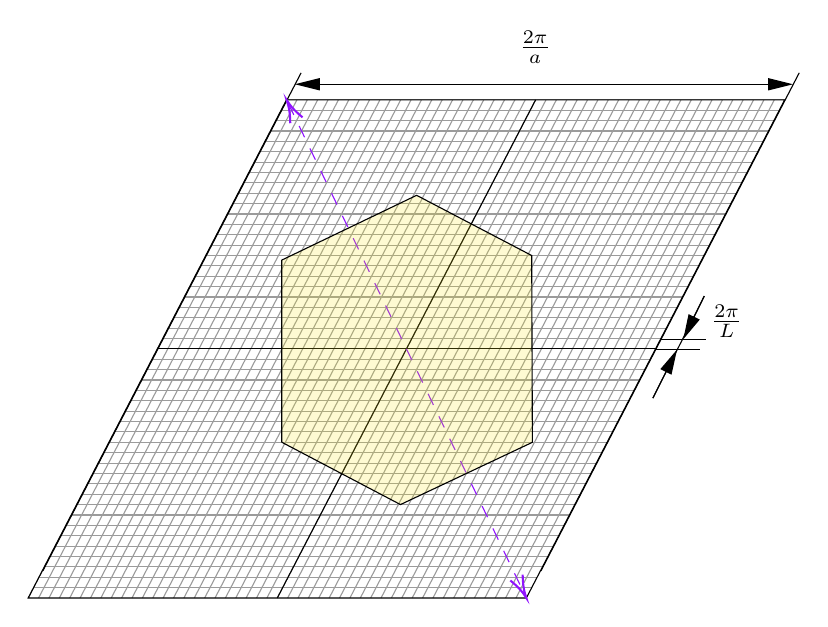
\begin{tikzpicture}[x=0.75pt,y=0.75pt,yscale=-1,xscale=1]
%uncomment if require: \path (0,370); %set diagram left start at 0, and has height of 370

%Shape: Grid [id:dp169871510593959] 
\draw  [draw opacity=0] (201,94.5) -- (441,94.5) -- (316.54,334.5) -- (76.54,334.5) -- cycle ; \draw  [color={rgb, 255:red, 155; green, 155; blue, 155 }  ,draw opacity=1 ] (201,94.5) -- (76.54,334.5)(206,94.5) -- (81.54,334.5)(211,94.5) -- (86.54,334.5)(216,94.5) -- (91.54,334.5)(221,94.5) -- (96.54,334.5)(226,94.5) -- (101.54,334.5)(231,94.5) -- (106.54,334.5)(236,94.5) -- (111.54,334.5)(241,94.5) -- (116.54,334.5)(246,94.5) -- (121.54,334.5)(251,94.5) -- (126.54,334.5)(256,94.5) -- (131.54,334.5)(261,94.5) -- (136.54,334.5)(266,94.5) -- (141.54,334.5)(271,94.5) -- (146.54,334.5)(276,94.5) -- (151.54,334.5)(281,94.5) -- (156.54,334.5)(286,94.5) -- (161.54,334.5)(291,94.5) -- (166.54,334.5)(296,94.5) -- (171.54,334.5)(301,94.5) -- (176.54,334.5)(306,94.5) -- (181.54,334.5)(311,94.5) -- (186.54,334.5)(316,94.5) -- (191.54,334.5)(321,94.5) -- (196.54,334.5)(326,94.5) -- (201.54,334.5)(331,94.5) -- (206.54,334.5)(336,94.5) -- (211.54,334.5)(341,94.5) -- (216.54,334.5)(346,94.5) -- (221.54,334.5)(351,94.5) -- (226.54,334.5)(356,94.5) -- (231.54,334.5)(361,94.5) -- (236.54,334.5)(366,94.5) -- (241.54,334.5)(371,94.5) -- (246.54,334.5)(376,94.5) -- (251.54,334.5)(381,94.5) -- (256.54,334.5)(386,94.5) -- (261.54,334.5)(391,94.5) -- (266.54,334.5)(396,94.5) -- (271.54,334.5)(401,94.5) -- (276.54,334.5)(406,94.5) -- (281.54,334.5)(411,94.5) -- (286.54,334.5)(416,94.5) -- (291.54,334.5)(421,94.5) -- (296.54,334.5)(426,94.5) -- (301.54,334.5)(431,94.5) -- (306.54,334.5)(436,94.5) -- (311.54,334.5) ; \draw  [color={rgb, 255:red, 155; green, 155; blue, 155 }  ,draw opacity=1 ] (201,94.5) -- (441,94.5)(198.41,99.5) -- (438.41,99.5)(195.81,104.5) -- (435.81,104.5)(193.22,109.5) -- (433.22,109.5)(190.63,114.5) -- (430.63,114.5)(188.04,119.5) -- (428.04,119.5)(185.44,124.5) -- (425.44,124.5)(182.85,129.5) -- (422.85,129.5)(180.26,134.5) -- (420.26,134.5)(177.66,139.5) -- (417.66,139.5)(175.07,144.5) -- (415.07,144.5)(172.48,149.5) -- (412.48,149.5)(169.89,154.5) -- (409.89,154.5)(167.29,159.5) -- (407.29,159.5)(164.7,164.5) -- (404.7,164.5)(162.11,169.5) -- (402.11,169.5)(159.51,174.5) -- (399.51,174.5)(156.92,179.5) -- (396.92,179.5)(154.33,184.5) -- (394.33,184.5)(151.74,189.5) -- (391.74,189.5)(149.14,194.5) -- (389.14,194.5)(146.55,199.5) -- (386.55,199.5)(143.96,204.5) -- (383.96,204.5)(141.36,209.5) -- (381.36,209.5)(138.77,214.5) -- (378.77,214.5)(136.18,219.5) -- (376.18,219.5)(133.59,224.5) -- (373.59,224.5)(130.99,229.5) -- (370.99,229.5)(128.4,234.5) -- (368.4,234.5)(125.81,239.5) -- (365.81,239.5)(123.21,244.5) -- (363.21,244.5)(120.62,249.5) -- (360.62,249.5)(118.03,254.5) -- (358.03,254.5)(115.44,259.5) -- (355.44,259.5)(112.84,264.5) -- (352.84,264.5)(110.25,269.5) -- (350.25,269.5)(107.66,274.5) -- (347.66,274.5)(105.06,279.5) -- (345.06,279.5)(102.47,284.5) -- (342.47,284.5)(99.88,289.5) -- (339.88,289.5)(97.29,294.5) -- (337.29,294.5)(94.69,299.5) -- (334.69,299.5)(92.1,304.5) -- (332.1,304.5)(89.51,309.5) -- (329.51,309.5)(86.91,314.5) -- (326.91,314.5)(84.32,319.5) -- (324.32,319.5)(81.73,324.5) -- (321.73,324.5)(79.14,329.5) -- (319.14,329.5) ; \draw  [color={rgb, 255:red, 155; green, 155; blue, 155 }  ,draw opacity=1 ]  ;
%Shape: Grid [id:dp6752969151127564] 
\draw  [draw opacity=0] (201,94.5) -- (441,94.5) -- (316.54,334.5) -- (76.54,334.5) -- cycle ; \draw   (321,94.5) -- (196.54,334.5) ; \draw   (138.77,214.5) -- (378.77,214.5) ; \draw   (201,94.5) -- (441,94.5) -- (316.54,334.5) -- (76.54,334.5) -- cycle ;

%Straight Lines [id:da9667181162257916] 
\draw    (208,81.5) -- (83.54,321.5) ;
%Straight Lines [id:da7305047384985015] 
\draw    (448,81.5) -- (323.54,321.5) ;
%Straight Lines [id:da1230438142218293] 
\draw    (207,87) -- (443,87) ;
\draw [shift={(445,87)}, rotate = 180] [fill={rgb, 255:red, 0; green, 0; blue, 0 }  ][line width=0.08]  [draw opacity=0] (12,-3) -- (0,0) -- (12,3) -- cycle    ;
\draw [shift={(205,87)}, rotate = 0] [fill={rgb, 255:red, 0; green, 0; blue, 0 }  ][line width=0.08]  [draw opacity=0] (12,-3) -- (0,0) -- (12,3) -- cycle    ;
%Straight Lines [id:da524967567110274] 
\draw    (377.47,238.23) -- (388.25,216.62) ;
\draw [shift={(389.14,214.83)}, rotate = 476.51] [fill={rgb, 255:red, 0; green, 0; blue, 0 }  ][line width=0.08]  [draw opacity=0] (12,-3) -- (0,0) -- (12,3) -- cycle    ;
%Straight Lines [id:da46717416425871905] 
\draw    (393.01,208.04) -- (402.27,189.03) ;
\draw [shift={(392.14,209.83)}, rotate = 295.97] [fill={rgb, 255:red, 0; green, 0; blue, 0 }  ][line width=0.08]  [draw opacity=0] (12,-3) -- (0,0) -- (12,3) -- cycle    ;
%Straight Lines [id:da7656127447329844] 
\draw    (381.27,209.83) -- (403,209.83) ;
%Straight Lines [id:da29332470867758964] 
\draw    (378.28,214.83) -- (400,214.83) ;
%Straight Lines [id:da3829083344578674] 
\draw    (377.47,238.23) -- (402.27,189.03) ;

%Straight Lines [id:da46787759331428336] 
\draw [color={rgb, 255:red, 144; green, 19; blue, 254 }  ,draw opacity=1 ] [dash pattern={on 4.5pt off 4.5pt}]  (258.77,214.5) -- (315.68,332.7) ;
\draw [shift={(316.54,334.5)}, rotate = 244.29000000000002] [color={rgb, 255:red, 144; green, 19; blue, 254 }  ,draw opacity=1 ][line width=0.75]    (10.93,-3.29) .. controls (6.95,-1.4) and (3.31,-0.3) .. (0,0) .. controls (3.31,0.3) and (6.95,1.4) .. (10.93,3.29)   ;
%Straight Lines [id:da9731434313195053] 
\draw [color={rgb, 255:red, 144; green, 19; blue, 254 }  ,draw opacity=1 ] [dash pattern={on 4.5pt off 4.5pt}]  (201.87,96.3) -- (258.77,214.5) ;
\draw [shift={(201,94.5)}, rotate = 64.29] [color={rgb, 255:red, 144; green, 19; blue, 254 }  ,draw opacity=1 ][line width=0.75]    (10.93,-3.29) .. controls (6.95,-1.4) and (3.31,-0.3) .. (0,0) .. controls (3.31,0.3) and (6.95,1.4) .. (10.93,3.29)   ;

%Straight Lines [id:da17199011984955814] 
\draw    (138.77,214.5) -- (258.77,214.5) ;
%Straight Lines [id:da3309278527701198] 
\draw    (198.77,171.67) -- (198.77,259.5) ;
%Shape: Polygon [id:ds11160849173424747] 
\draw  [fill={rgb, 255:red, 248; green, 231; blue, 28 }  ,fill opacity=0.2 ] (263.66,140.5) -- (319.11,169.5) -- (319.44,259.5) -- (255.88,289.5) -- (198.77,259.5) -- (198.77,171.67) -- cycle ;

% Text Node
\draw (312,60) node [anchor=north west][inner sep=0.75pt]    {$\frac{2\pi }{a}$};
% Text Node
\draw (404.27,192.03) node [anchor=north west][inner sep=0.75pt]    {$\frac{2\pi }{L}$};


\end{tikzpicture}

    \caption{三种动量空间,倒格子(黑色)和由于晶体是有限大小的而产生的晶格常数为$2\pi / L$的离散动量点阵(灰色),两者均可以无限延伸;第一布里渊区用淡黄色标记,它的边界垂直平分的倒格矢包括诸$\vb*{b}_i$以及用紫色标出的倒格矢}
\end{figure}

现在我们有三种动量空间,这三种动量空间、它们适用于什么样的函数以及它们对应的傅里叶变换列举如下。
在这里唯一确定的是坐标空间的场算符$\psi(\vb*{r})$,它满足
\[
    \comm*{\psi_\alpha(\vb*{r})}{\psi^\dagger_\beta(\vb*{r}')} = \delta_{\alpha \beta} \delta(\vb*{r} - \vb*{r}').
\]
实际上由于我们局限在一个大小为$V$的盒子中,这里的$\delta(\vb*{r} - \vb*{r}')$函数并非全空间中的$\delta$函数,而是实空间区域$V$中的$\delta$函数,它能够让任何限制在$V$中的函数$f(\vb*{r})$满足
\[
    \int_V \dd[3]{\vb*{r}'} f(\vb*{r}') \delta(\vb*{r} - \vb*{r}') = f(\vb*{r}).
\]
但显然$V \to \infty$时这种“软化”的$\delta(\vb*{r} - \vb*{r}')$就趋于无限大空间中的$\delta(\vb*{r} - \vb*{r}')$,从而以下我们可以混用两种$\delta(\vb*{r} - \vb*{r}')$。
动量表象的归一化系数是不确定的。
我们需要定义电子波函数的内积,由于$\braket*{\psi}{\psi} = 1$,每种内积定义都会在波函数前面引入一个不同的归一化因子。
归一化是很重要的,因为诸如微扰论给出的能级修正等在归一化不对时是不正确的;此外一些物理量真的会正比于$V$或者说$N$,从而归一化常数中的$V$或是$N$是很重要的。

\begin{enumerate}
    \item 晶格常数为$2\pi / L$的三维点阵是被限制在边长为$L$的实空间方盒中的函数的傅里叶变换的动量取值范围,由于$L$通常很大,这个点阵要比倒格子密得多,在倒格子的尺度上工作时没有必要考虑晶格常数为$2\pi / L$的三维点阵是离散的这一事实。
    该三维点阵动量空间虽然是离散的,却是无限大的,因为它实际上给出的是一个箱子中所有可能的平面波的波矢,而这当然可以取到无限大。
    与这个动量空间相关的傅里叶变换的归一化表达式为
    \begin{equation}
        \frac{1}{V} \int_V \dd[3]{\vb*{r}} \ee^{\ii (\vb*{k} - \vb*{k}') \cdot \vb*{r}} = \delta_{\vb*{k} \vb*{k}'}, \quad \frac{1}{V} \sum_{\vb*{k}} \ee^{\ii \vb*{k} \cdot (\vb*{r} - \vb*{r}')} = \delta(\vb*{r} - \vb*{r}'),
    \end{equation}
    第二个表达式中的$\delta$函数就是动量空间无限大的一个结果。于是有以下几种方案:一种是将动量本征态取为
    \begin{equation}
        \psi_{\vb*{k}}(\vb*{r}) = \frac{1}{\sqrt{V}} \ee^{\ii \vb*{k} \cdot \vb*{r}},
    \end{equation}
    则容易验证我们应该定义内积为
    \begin{equation}
        \braket*{\alpha}{\beta} = \int \dd[3]{\vb*{r}} \braket*{\alpha}{\vb*{r}} \braket*{\vb*{r}}{\beta} = \sum_{\vb*{k}} \braket*{\alpha}{\vb*{k}} \braket*{\vb*{k}}{\beta},
        \label{eq:integrate-ouver-whole-space}
    \end{equation}
    这样可以满足归一化条件。此时表象变换为
    \[
        \braket*{\vb*{k}}{\alpha} = \int \dd[3]{\vb*{r}} \frac{1}{\sqrt{V}} \ee^{- \ii \vb*{k} \cdot \vb*{r}} \braket*{\vb*{r}}{\alpha}, \quad \braket*{\vb*{r}}{\alpha} = \sum_{\vb*{k}} \frac{1}{\sqrt{V}} \ee^{ \ii \vb*{k} \cdot \vb*{r}} \braket*{\vb*{k}}{\alpha}
    \]
    于是通常如此定义傅里叶变换:
    \begin{equation}
        f(\vb*{k}) = \frac{1}{\sqrt{V}} \int \dd[3]{\vb*{r}} \ee^{- \ii \vb*{k} \cdot \vb*{r}} f(\vb*{r}), \quad f(\vb*{r}) = \frac{1}{\sqrt{V}} \sum_{\vb*{k}} \ee^{\ii \vb*{k} \cdot \vb*{r}} f(\vb*{k}),
        \label{eq:sqrt-v-rep}
    \end{equation}
    这样定义的好处在于,我们知道${\psi}^\dagger(\vb*{r})$和${c}^\dagger_{\vb*{k}}$彼此为傅里叶变换,而如果采用上式的傅里叶变换定义,那么从
    \[
        \acomm*{{\psi}_\alpha(\vb*{r})}{{\psi}^\dagger_\beta(\vb*{r}')} = \delta(\vb*{r}-\vb*{r}') \delta_{\alpha \beta}
    \]
    可以得到
    \[
        \acomm*{{c}_{\vb*{k}\alpha}}{{c}^\dagger_{\vb*{k}' \beta}} = \delta_{\vb*{k} \vb*{k}'} \delta_{\alpha \beta},
    \]
    于是动量表象下的产生湮灭算符关系也是非常简单的。
    
    另一种方案是取动量本征态为
    \begin{equation}
        \psi_{\vb*{k}}(\vb*{r}) = \ee^{\ii \vb*{k} \cdot \vb*{r}},
    \end{equation}
    此时内积应该定义为
    \begin{equation}
        \braket*{\alpha}{\beta} = \frac{1}{V} \int \dd[3]{\vb*{r}} \braket*{\alpha}{\vb*{r}} \braket*{\vb*{r}}{\beta} = \frac{1}{V} \sum_{\vb*{k}} \braket*{\alpha}{\vb*{k}} \braket*{\vb*{k}}{\beta}, 
        \label{eq:integrate-ouver-whole-space-divided}
    \end{equation}
    这样的好处在于,在$V$很大时,考虑到点阵的晶格常数为$2\pi / L$,可以做替换
    \begin{equation}
        \frac{1}{V} \sum_{\vb*{k}} \longrightarrow \int \frac{\dd[3]{\vb*{k}}}{(2\pi)^3},
    \end{equation}
    从而$\vb*{k}$基底下实际上没有$V$的依赖,正如动量本征态的定义所展示的那样。此时表象变换为
    \[
        \braket*{\vb*{r}}{\beta} = \frac{1}{V} \sum_{\vb*{k}} \ee^{\ii \vb*{k} \cdot \vb*{r}} \braket*{\vb*{k}}{\beta} = \int \frac{\dd[3]{\vb*{k}}}{(2\pi)^3} \ee^{\ii \vb*{k} \cdot \vb*{r}} \braket*{\vb*{k}}{\beta}, \quad 
    \]
    从而傅里叶变换应该取为
    \begin{equation}
        f(\vb*{r}) = \frac{1}{V} \sum_{\vb*{k}} \ee^{\ii \vb*{k} \cdot \vb*{r}} f(\vb*{k}) = \int \frac{\dd[3]{\vb*{k}}}{(2\pi)^3} \ee^{\ii \vb*{k} \cdot \vb*{r}} f(\vb*{k}).
        \label{eq:v-rep}
    \end{equation}
    此时
    \begin{equation}
        \comm*{c_{\vb*{k} \alpha}}{c_{\vb*{k}' \beta}^\dagger} = (2\pi)^3 \delta_{\alpha \beta} \delta_{\vb*{k} \vb*{k}'}.
    \end{equation}
    在这种记号下对$2n$个坐标空间下的场算符的乘积积分,所得结果用动量空间中的产生湮灭算符表示则一定正比于$V$,因为到最后那个对$\vb*{r}$的积分给出
    \[
        \int \dd[3]{\vb*{r}} \ee^{\ii \sum \vb*{k} \cdot \vb*{r}} \propto V.
    \]
    相反,在\eqref{eq:sqrt-v-rep}的记号下,对$2n$个坐标空间下的场算符的乘积积分,所得结果用动量空间中的产生湮灭算符表示则正比于$V^{1 - n}$。
    \eqref{eq:sqrt-v-rep}相当于将体积依赖放到了与动量空间有关的物理量(比如说$\psi_{\vb*{k}}$)中,而\eqref{eq:v-rep}相当于将体积依赖放到了与坐标空间有关的物理量(主要是对$\dd[3]{\vb*{r}}$积分时总是需要乘以$V$)中。
    我们通常采用第一种记号,也就是\eqref{eq:sqrt-v-rep},因为在固体物理中实空间的物理定律——如库仑定律——是保证和自由情况下完全一样的。例如我们时常需要从库伦相互作用获得某种等效相互作用通道,那么使用记号\eqref{eq:sqrt-v-rep}的话就不需要担心归一化出错。

    有时候,我们不使用平面波基底展开波函数,但是这并不影响$\vb*{r}$,即内积定义\eqref{eq:integrate-ouver-whole-space}和\eqref{eq:integrate-ouver-whole-space-divided}中涉及坐标的部分在任何时候都是可以用的。
    我们通常还是使用\eqref{eq:integrate-ouver-whole-space}。

    \item 倒格子是具有和晶格一样的周期性的连续函数的傅里叶变换的动量取值范围。与之相关的归一化表达式为
    \begin{equation}
        \frac{1}{V_\text{u.c.}} \int_{V_\text{u.c.}} \dd[3]{\vb*{r}} \ee^{\ii \vb*{r} \cdot (\vb*{k} - \vb*{k}')} = \delta_{\vb*{k} \vb*{k}'}, \quad \frac{1}{V_\text{u.c.}} \sum_{\vb*{k}} \ee^{\ii \vb*{r} \cdot (\vb*{k} - \vb*{k}')} = \delta(\vb*{r} - \vb*{r}'), 
        \label{eq:normalization-periodic}
    \end{equation}
    其中$\vb*{k}$取遍整个倒格子而$\vb*{r}$取遍一个正格子晶胞内部的所有点(因为仅讨论周期函数)。这里我们使用$V_\text{u.c.}$表示一个正格子晶胞的大小,来和整块晶体的大小区分开。相应的,傅里叶变换为
    \begin{equation}
        f(\vb*{k}) = \frac{1}{\sqrt{V_\text{u.c.}}} \int \dd[3]{\vb*{r}} \ee^{- \ii \vb*{k} \cdot \vb*{r}} f(\vb*{r}), \quad f(\vb*{r}) = \frac{1}{\sqrt{V_\text{u.c.}}} \sum_{\vb*{k}} \ee^{\ii \vb*{k} \cdot \vb*{r}} f(\vb*{r}).
    \end{equation}
    倒格子是无限大的,因此以上展示的傅里叶变换的动量空间同样是无限大的。
    \item 倒空间的原胞,如第一布里渊区,是定义在正格子上的函数的傅里叶变换的动量取值范围。归一化表达式为
    \begin{equation}
        \frac{1}{N} \sum_{\vb*{a}_i} \ee^{\ii (\vb*{k} - \vb*{k}') \cdot \vb*{a}_i} = \delta_{\vb*{k} \vb*{k}'}, \quad \frac{1}{N} \sum_{\vb*{k}} \ee^{\ii (\vb*{a}_i - \vb*{a}_j) \cdot \vb*{k}} = \delta_{ij}.
    \end{equation}
    第二个表达式表明对定义在正格子上的函数,它在动量空间中在一个倒空间原胞中的动量取值有$N$个。傅里叶变换为
    \begin{equation}
        f(\vb*{k}) = \frac{1}{\sqrt{N}} \sum_{i} \ee^{- \ii \vb*{k} \cdot \vb*{a}_i} f(i), \quad f(i) = \frac{1}{\sqrt{N}} \sum_{\vb*{k}} \ee^{\ii \vb*{k} \cdot \vb*{a}_i} f(\vb*{k}),
        \label{eq:lattice-fourier}
    \end{equation}
    即我们将动量本征态取为
    \begin{equation}
        \psi_{\vb*{k}}(i) = \frac{1}{\sqrt{N}} \ee^{\ii \vb*{k} \cdot \vb*{a}_i},
    \end{equation}
    从而内积应该定义为
    \begin{equation}
        \braket*{\alpha}{\beta} = \sum_i \braket*{\alpha}{i} \braket*{i}{\beta} = \sum_{\vb*{k}} \braket*{\alpha}{\vb*{k}} \braket*{\vb*{k}}{\beta}
        \label{eq:sum-over-lattice}
    \end{equation}
    以满足归一化条件。
    使用这种记号和\eqref{eq:sqrt-v-rep}类似,一个对$2n$个坐标空间中的场算符乘积求和的项如果改用$c_{\vb*{k}}$表示,将正比于$N^{1-n}$。
    与前两种情况不同,上式中的动量空间中只有有限个(共$N$个)动量。实际上容易验证,这$N$个动量恰恰是一个倒空间原胞中容纳的全部来自晶格常数为$2\pi / L$的点阵的格点。
    这样,我们就有
    \[
        N = \frac{2\pi / V_\text{u.c.}}{2\pi / V},
    \]
    即
    \begin{equation}
        V = N V_\text{u.c.},
    \end{equation}
    正好是预期中的结果。在热力学极限下$N \to 0$,此时倒空间原胞中容纳的动量取值趋于连续。这就是前述“在倒格子的尺度上工作时无需考虑晶体有限大(即$L$有限大)导致的动量离散化”的一个直观理解。
\end{enumerate}

还有一个应该注意的细节:以上推导中我们都使用了$\delta_{\vb*{k} \vb*{k}'}$,一些时候也会把它写成$\delta(\vb*{k}- \vb*{k}')$,从而和坐标空间保持一致,但是要注意,如果我们希望$\delta(\vb*{k} - \vb*{k}')$满足
\[
    \int \dd[3]{\vb*{k}} \delta(\vb*{k} - \vb*{k}') f(\vb*{k}) = f(\vb*{k}'),
\]
那么其实应该取
\begin{equation}
    \delta(\vb*{k} - \vb*{k}') = \frac{V}{(2\pi)^3} \delta_{\vb*{k} \vb*{k}'} , \quad \text{as $V \to \infty$}.
\end{equation}

\section{晶体的对称性和分类}

\subsection{晶体结构分类概述}\label{sec:crystal-structure-intro}

从本节开始我们尝试用对称性分类晶体。晶体的对称性是欧氏空间的等距变换群作用在离散格子上的一个子群,其中的任何一个元素可以标记为$(R|\vb*{a})$,其中$R$表示一个不包括平移的等距变换(有限大小的对象的对称群只包括这种变换,因为有限大小的对象不可能具有平移对称性),$\vb*{a}$表示平移的距离。

晶体的对称性是非常有用的,例如,它可以直接用于决定晶体的一些参数的形式。例如,对立方晶体,介电张量是一个标量,而对六角晶体介电张量具有
\[
    \pmqty{\dmat{\epsilon_\parallel, \epsilon_\bot, \epsilon_\bot}}
\]
的形式。晶体分为晶格和基元,而晶格的对称性是具有这种晶格的晶体能够具有的最高对称性(即基元具有球对称性时晶体具有的对称性)——如果基元在某种不改变晶格的操作下会发生改变,那么整个晶体的对称性实际上低于晶格的对称性。
例如,金刚石和闪锌矿具有完全一样的晶格,但是金刚石基元具有沿着化学键中心的反射对称性,而闪锌矿则没有。 %TODO
因此,我们可以首先分析晶格的对称性,然后考虑基元的对称性而得到不考虑平移的晶体的对称性,最后加入平移(它是空间群的不变子群)而得到完整的对称性。

我们汇总一下所有的分类:
\begin{enumerate}
    \item \concept{晶系},这是最为粗疏的分类方法,其依据是晶格的对称轴和对称面的数目,共有7种晶系。晶系给定之后晶格的点群(见下文)可以不同,而可以验证,如果两种晶体分别属于不同的晶系,这两种晶体的点群肯定是不一样的。
    晶系提供了晶格的点群,是具有这种晶格的晶体可以具有的最大点群(如果基元对称性较低,实际的晶体点群会小于晶格的点群)。
    \item \concept{布拉伐晶格},在每种晶系内,按照一个晶体学单胞(默认8个角上都有格点)中各个格点的位置——简单,面心,体心,底心(共三种)——可以细分出总计14种布拉伐格子。%
    \footnote{
        角上的格点以外的格点不能位于简单、面心、体心、底心以外的地方,否则我们总是可以通过重新定义基元来把晶体划归到简单、面心、底心中的一类中去。
    }%
    虽然表面上应该有$7 \cdot 6 = 42$种格子,但其中很大一部分是重复的。
    在晶系给定之后,布拉伐格子额外提供了关于平移对称性的信息。
    因此,布拉伐格子概括了\emph{晶格}的对称性:给定一个布拉伐格子类型,对应的晶格的空间对称群就可以写下来了。
    \item \concept{晶体点群}或者简称\concept{点群},虽然后者也常被用于指代一个更大的概念,指保持空间中一个点不动的群,实际上就是描述有限大小的物体的对称性的群。
    一个晶体群(即晶体的完整对称性,见下文)中除了平移以外的部分一定是$O(3)$的子群,可以写成某个坐标系下的一个矩阵群,矩阵变换下坐标原点始终是不动的,因此点群一定会保持一个点不动,这个点就是如前所述的原点;除此以外的其它点在某个群操作下都会发生变动。
    晶体点群一定是广义上的点群。然而,并非所有广义上的点群都是晶体点群,因为它们可能会和空间平移不兼容。
    一个晶体的点群一定是它的晶系的点群的子群。晶体点群和它的晶系的点群之间的差异表达了基元有多不对称。
    在晶系给定之后,晶体点群和布拉伐格子类型(简单、体心、面心、底心)可以任意组合,彼此无关。
    \item \concept{晶体群}或者说\concept{晶体空间群},最为细致的晶体对称性分类,它是欧氏空间$\mathbb{R}^n$的离散等距变换子群,并且$\mathbb{R} / G$是紧致的(即整个空间中任何一个点都可以等效到某个晶胞中)。
    数学上可以证明这样的群一定包含$n$种彼此独立的平移变换(本该如此,因为我们需要这些平移变换来产生完整的布拉伐格子),具体这些平移变换是什么由布拉伐格子的类型决定。
    在晶体点群和布拉伐格子均给定之后仍然不能完全确定晶体空间群,因为一些复式晶格的点群操作和平移操作一起使用时,部分点群操作并不在基元的点群中,然而,先做它们然后附带小的平移操作却能够保持晶体不变。
    实际上,这意味着“点群”的概念宏观和微观来看会有微妙的不同:典型的例子是金刚石和ZnS晶体,两者都是复式晶格,但是金刚石的几何上不等价的两种格点含有一样的原子,因此,虽然两种晶体的微观点群都是$T_d$,对金刚石,$O_h$点群中不是$T_d$的那些操作如果与一段很小的平移结合,仍然可以保持晶体不变,因此宏观地看,金刚石似乎在$O_h$点群下也不变。
\end{enumerate}

\subsection{点群中的变换}

我们来分析点群中可能出现的变换。
首先肯定有旋转,并且由于我们讨论的是离散对象上的对称群,旋转一定是离散旋转,即绕着某个轴,一次旋转$2\pi / n$,$n$为某个整数。
这样的旋转操作构成一个点群的子群,记作$C_{n}$,相应的转轴称为一条\concept{$C_{n}$轴};一个转角为$2\pi k / n$的离散旋转操作记作$c_n^k$。
其次肯定还有\concept{空间反演}或者说\concept{反射},这包括镜面反射和点反演。我们用$\sigma$标记一个反演平面,用$i$标记一个反演点。
在给定一条已知的旋转轴之后,将垂直于它的反演平面记作$\sigma_h$,将包含它的反演平面记作$\sigma_\nu$;如果给定两条对称轴而有一个反演平面正好平分这个角,那么这个反演平面就是$\sigma_d$。
这两个符号也用于指代对应的空间反演操作。
简单考虑一下会发现这些操作和它们的乘积足够给出所有可能的点群变换。

由于讨论范围局限于一个点群,总是存在一个点,在所有变换下都不变。
因此,一个点群内的旋转操作的旋转轴一定有共同的交点,这个交点就是反演中心,反演平面一定包含这个点。

空间反演和反射操作并非简单地被直积在一起——它们之间会有一些特殊的代数关系。
例如,很明显在给定一条旋转轴之后,$c_n^k$,$\sigma_h$和$\sigma_\nu$之间会有某些特殊的代数关系。
我们将$z$轴取在旋转轴上,则
\begin{equation}
    c_n^k = \pmqty{\dmat{ \cos(\frac{2\pi k}{n}) & -\sin(\frac{2\pi k}{n}) \\ \sin(\frac{2\pi k}{n}) & \cos(\frac{2\pi k}{n}), 0 }},
\end{equation}
而
\begin{equation}
    \sigma_h = \pmqty{\dmat{1, 1, -1}}, \quad i = \pmqty{\dmat{-1, -1, -1}},
\end{equation}
于是立刻可以看出
\begin{equation}
    c_n^k \sigma_h = \sigma_h c^n_k.
\end{equation}
在$n=2$时$C_2=\{e, c^1_2\}$,记$c^1_2$为$c_2$,则
\begin{equation}
    c_2 = \pmqty{\dmat{-1, -1, 1}},
\end{equation}
计算可得
\begin{equation}
    c_2 \sigma_h = \sigma_h c_2 = i, \quad c_2 i = i c_2 = \sigma_h, \quad \sigma_h i = i \sigma_h = c_2.
    \label{eq:sigma-c-i}
\end{equation}

假定有两个二阶轴$C_{2A}$和$C_{2B}$交于$O$点,它们之间的夹角为$\varphi$,则
\begin{equation}
    c_{2A} c_{2B} = c(2\varphi),
\end{equation}
其中$c(2\varphi)$的旋转轴垂直于$C_{2A}$和$C_{2B}$确定的平面。
这件事只需要通过
\begin{equation}
    c_{2B} = c(\varphi) c_{2A} c(-\varphi)
    \label{eq:ab-axis-phi-rotation}
\end{equation}
即可得到证明。类似地可以证明
\begin{equation}
    c_{2B} c_{2A} = c(-2\varphi).
    \label{eq:cb-ca-phi-axis}
\end{equation}

也可以对反射面证明类似的公式。设有两个反射面$\sigma_{\nu}$和$\sigma'_\nu$相交于$z$轴,以$z$轴为旋转轴,则有
\begin{equation}
    \sigma'_\nu \sigma_\nu = c(2\varphi), \quad \sigma_\nu \sigma'_\nu = c(-2\varphi).
\end{equation}
证明方法是,取和$\sigma_{\nu}$垂直的$C_2$轴$c_2$,和$\sigma'_\nu$垂直的$C_2$轴$c'_2$,则有
\[
    \sigma_\nu = c_2 i = i c_2, \quad \sigma'_\nu = c'_2 i = i c'_2,
\]
于是
\[
    \sigma'_\nu \sigma_\nu = c_2' c_2 = c(2\varphi).
\]

\eqref{eq:ab-axis-phi-rotation}其实说明一件事:一个旋转轴在特定的对称操作下可以被转换成另一个旋转轴。
我们先讨论这“特定的对称操作”是另一个旋转的情况。
设一个$C_n$轴和一个$C_m$轴相交于$O$点,两者夹角为$\varphi$,则可以获得这样的新的旋转:
\[
    c_n^j c_m^i (c_n^j)^{-1},
\]
因此通过绕着$C_n$轴的旋转可以产生$n$个$C_m$轴,记作$C_{m j}$,其中的操作为
\begin{equation}
    c_{m j}^i = c_n^j c_m^i (c_n^j)^{-1}.
    \label{eq:from-one-axis-to-another}
\end{equation}
特别的,如果有一个$C_2$轴与$C_m$轴垂直,有
\begin{equation}
    c_n^{-k} = c_2 c_n^k c_2.
    \label{eq:inverse-k-c2}
\end{equation}
可以验证,将旋转轴和$\sigma$面做共轭变换也能够得到新的旋转,即
\[
    \sigma c_m^i \sigma
\]
也是一个$C_m$操作,记为$C_m'$,并且可以证明$C_m$的正转被映射为了绕着$C_m'$的反转,即
\begin{equation}
    {c'_{m}}^{-k} = \sigma c_m^k \sigma.
\end{equation}
特别的,
\begin{equation}
    \sigma_\nu c_m^k \sigma_\nu = c_2 i c_m^k i c_2 = c_2 c_m^k c_2 = c_m^{-k},
\end{equation}
而对$\sigma_h$有
\begin{equation}
    c_n^k = \sigma_h c_n^k \sigma_h.
    \label{eq:perpendicular-sigma-c}
\end{equation}
看起来这里似乎有一个矛盾,因为等式左边的$k$应该是$-k$,但是在$\sigma$是$\sigma_h$时变换前后的旋转轴其实是同一根旋转轴,只不过指向相反,那么如果将它们看成同一根轴,就应该将$-k$换成$k$。
旋转操作在点反演的共轭变换下不变,即
\begin{equation}
    i c_m^k i = c_m^k.
\end{equation}
以上方程给出了$c_m^k$在各种共轭变换下的变换,从而给出了一个旋转操作的等价类。
给定一个旋转轴和它的旋转群,做这些共轭变换,会得到另一个旋转群,从而以上方程实际上指出了一个点群中的\concept{等价旋转轴}:对一条旋转轴$C_m$,如果有和它相交的旋转轴$C_n$,那么$C_m$中的等价旋转轴包括$C_{mj}$,$j$取遍$0$到$n-1$;如果有反演面,那么就有等价旋转轴$C_m'$;如果有与之垂直的$C_2$轴,那在$C_m$的旋转群内部就有群元彼此等价。
没有更多方式产生等价旋转轴。需注意两个轴等价不代表以它们为轴的所有旋转操作都在一个等价类中;这只能说明,某个绕一个轴的旋转一定和某个绕另一个轴的旋转等价。

也可以依照类似的方法分析反射变换的共轭等价类。对反演面,做旋转的共轭变换有
\begin{equation}
    \sigma' = c_n^k \sigma c_n^{-k}.
\end{equation}

\subsection{点群的分类}

本节给出所有可能的晶体点群,以及如何分类它们。

\subsubsection{第一类点群} 

\concept{第一类点群}包括那些只有纯粹的转动,即没有反演的点群。它们也可以称为离散旋转群。
第一类点群中最简单的是\concept{单轴点群},即只有一条对称轴的点群,它们就是$C_n$。
$C_n$是$n$阶阿贝尔群,从而有$n$个不可约表示,每个不可约表示都是一维的。
晶体点群必须和离散空间平移对称性兼容,换而言之,做完晶体点群变换之后的晶格必须仍然是原来的晶格,格矢的指向不变。
正是这个条件导致$C_n$中的$n$不能任意取值。分子点群就不受到这个限制。
设$\vb*{t}$是一个长度最短的格矢(我们正是在这一步用到了“存在一个晶格”的假设,否则没有一个长度最短但是有限的格矢),我们以它的起点为中心施加一个点群中的转动$c_n^1$,则在转动$c_n^1$之后它必须变成另一个格矢,这等价于说$\vb*{t}' - \vb*{t}$是一个格矢。
我们有
\[
    \abs*{\vb*{t}' - \vb*{t}} = 2 \abs*{\vb*{t}} \sin\left(\frac{\pi}{n}\right),
\]
由于$\vb*{t}$长度最短,有
\[
    2 \abs*{\vb*{t}} \sin\left(\frac{\pi}{n}\right) \geq \abs*{\vb*{t}},
\]
于是$n$只能从下面的值中选取:
\[
    n = 1, 2, 3, 4, 6.
\]
我们会发现每个值都是可以的:$n=1$对应一个平庸的情况,即晶体没有什么特别的点群对称性;$C_2$和$C_4$可以和正方形晶格兼容,$C_3$可以和三角晶格兼容,$C_6$可以和蜂窝晶格兼容。
总之,晶体点群中,单轴点群只有$C_1, C_2, C_3, C_4, C_6$,这就是所谓的\concept{晶体局限定理}。
实际上,点群同样会选择能够与它搭配的晶格,晶格的形状不能完全任意搭配,一些点群只能和特定的一些晶格一起出现。

另一种第一类点群不包含或者只包含一个高阶轴,除此以外的旋转轴都是$C_2$轴。
如果有两个$C_2$轴,那么它们必须垂直,否则按照\eqref{eq:cb-ca-phi-axis}就会产生高阶轴(证明\eqref{eq:cb-ca-phi-axis}时我们是假定存在垂直两根$C_2$轴的轴,但是这没有关系,因为群乘法的封闭性保证了$c_{2A}$和$c_{2B}$相乘的结果总是在原来的点群中)。
在两根$C_2$轴垂直时,围绕它们旋转$\pi$的操作相乘给出绕着垂直于这两根轴确定的平面旋转$\pi$的操作。
因此我们得到一个点群$D_2$。无法再塞入更多的$C_2$轴了——三维空间中彼此相互正交的方向最多能有三个。因此,$D_2$就是只含有$C_2$轴但是和$C_n$不同的唯一一个第一类点群。

现在考虑一个只有一个$C_n$高阶轴的第一类点群,剩下的旋转轴只有$C_2$轴。这些$C_2$轴必须和$C_n$轴垂直,否则根据\eqref{eq:from-one-axis-to-another}将会有两条$C_n$轴。
反过来,通过$c_n^k$共轭变换,从一条$C_2$轴可以产生$n$个$C_2$轴。不能有更多的$C_2$轴了,否则将会出现另一条和$C_n$轴重合的高阶轴。
于是我们又得到了一个点群,它包含一条$C_n$轴和$n$条与之垂直,相邻夹角为$\pi / n$的$C_2$轴(注意这$n$条轴都是直线而不是射线,从而,相邻的$C_2$轴的夹角是$2\pi/2n$)。记这样的群为$D_n$,其阶为$2n$,其中有$C_n$轴给出的$n$个(包含了单位元的)操作和$n$个$C_2$轴给出的旋转$\pi$的操作。
$C_2$轴旋转和$C_n$轴旋转的复合给出的也是$C_2$轴旋转。
可以看出$D_n$实际上就是正$n$边形的对称群。
由于$C_n$中的$n$有限制,因此只有$D_1, D_2, D_4, D_6$能成为晶体点群。

这些$D_n$群的等价类划分可以如下做出。容易验证在$D_n$中,我们有
\[
    c_2 c_2' c_2 = c_2', \quad c_n^k c_2 c_n^{-k} = c_2', \quad c_2 c_n^k c_2 = c_n^{-k}, \quad c_n^k c_n^{k'} c_n^{-k} = c_n^{k'},
\]
因此$D_n$的一个等价类中要么都是$C_n$旋转,要么都是$C_2$旋转。上式直接给出$C_n$的分类:$c_n^{k}$和$c_n^{-k}$被分为一类。
我们发现$c_n^1 c_2 c_n^{-1}$和$c_2$的夹角为$2\pi/n$,即通过$c_n^k$对$c_2$做共轭变换,一次最少导致$2\pi/n$的方向变化。
这意味着,如果$n$是偶数,那么通过$c_n^k$对$c_2$做共轭变换只能够覆盖一半的$C_2$轴,因此全体$C_2$轴被分成两个等价类;而对奇数$n$通过$c_n^k$对$c_2$做共轭变换可以覆盖一半的$C_2$轴。
总之,对奇数$n$,等价类包括:单位元,全体$C_2$轴作为一个等价类,以及
\[
    (c_n^1, c_n^{n-1}), \ \  \ldots, \ \  (c_n^{(n-1)/2}, c_n^{(n+1)/2})
\]
共计$(n+3)/2$个;而对偶数$n$,等价类包括:单位元,两个包含了$C_2$轴的等价类,以及
\[
    (c_n^1, c_n^{n-1}), \ \  \ldots, \ \  (c_n^{n/2-1}, c_n^{n/2+1}), \ \ c_n^{n/2},
\]
共计$3+n/2$个。这些等价类的数目就是不可约表示的数目,而全体不可约表示的维数的平方和就是群的阶,于是不可约表示的维数确定如下:
\begin{itemize}
    \item $D_2$有$4$个$1$维表示;
    \item $D_3$有$2$个$1$维表示,$1$个$2$维表示;
    \item $D_4$有$4$个$1$维表示,$1$个$2$维表示;
    \item $D_6$有$4$个$1$维表示,$2$个$2$维表示。
\end{itemize}

最后我们考虑具有多个高阶轴的第一类点群。设有两根高阶轴相交于$O$点,分别为$C_m$轴和$C_n$轴,并且它们之间的夹角最小。
使用之前的套路,可以获得环绕在$C_n$轴周围的$n$根$C_m$轴,以及环绕在$C_m$轴周围的$m$根$C_n$轴。接着我们从中再次挑选出一对夹角最小的$C_m$轴和$C_n$轴,重复这个步骤。
晶体点群的有限性和封闭性意味着这种迭代最终会停止。一点几何上的直觉就告诉我们,这样产生的全体对称轴和一个以$O$为球心的球面的交点连接起来将会产生一个正多面体。
因此,具有多个高阶轴的第一类点群必须包括某个正多面体的全部旋转对称性。
由于正多面体的高度对称性,实际上无法向正多面体的旋转对称群中再塞入更多的旋转对称性而仍然得到一个离散旋转群。因此具有多个高阶轴的第一类点群一定是某个正多面体的旋转对称群。

于是我们首先分析正多面体的对称性。一共只有五种正多面体,其中正四面体的旋转对称群是$T$,正八面体和立方体的旋转对称群是$O$,正二十面体和正十二面体的旋转对称群是$I$,但是$I$含有一个$C_5$轴,因此不能作为晶体点群。
因此,具有多个高阶轴的第一类点群必须包括$T$或$O$。
$T$群是12阶群,具有四个$C_3$轴和三个$C_2$轴。可以验证$C_3$轴彼此等价,$C_2$轴彼此等价,等价类为$e$,全体$c_2$,全体$c_3^1$和全体$c_3^2$,共4个等价类,从而有3个1维不可约表示和1个3维不可约表示。
$O$群是24阶群,有三个$C_4$轴,四个$C_3$轴和六个$C_2$轴,容易验证所有$C_4$轴都是等价的,所有$C_3$轴和$C_2$轴也是等价的,并且每个高阶轴都有与之垂直的$C_2$轴,从而正转和反转相同角度的旋转操作也是等价的。
这样,等价类包括:单位元,全体$c_2$,全体$c_3^1$和全体$c_3^2$构成的单独一个类,全体$c_4^1$和全体$c_4^3$构成的一个类,全体$c_4^2$,共计5个等价类。

总之,我们得到了11种第一类点群:
\[
    C_1, C_2, C_3, C_4, C_6, D_2, D_3, D_4, D_6, T, O.
\]

\subsubsection{第二类点群} 

现在将反演操作加入。点群中的旋转部分组成一个正规子群,从而,第二类点群可以通过向第一类点群加入反演操作来得到。
实际上容易发现如果点群中包括$i$,那么$\{e, i\}$也是一个正规子群。
能够加入的反演操作包括面反演操作和中心反演操作。
向非平凡的旋转群加入面反演操作$\sigma$时,如果反射面和一个对称轴既不垂直也没有包含关系,则显然会产生一条新的对称轴,新的对称轴根据\eqref{eq:from-one-axis-to-another}又可以产生新的对称轴。
新的对称轴或是可以没完没了地产生,这样得到的就不是有限大小的点群了,或是在产生一定数目的新对称轴之后停下,此时$\sigma$或者必须能够让某个对称轴不变,或者让两个对称轴相互转化(几何上的考虑表明,不可能让多个对称轴做置换)。
如果反演操作总是将一个对称轴转化为另一个对称轴(并且与此同时让后者也变成前者),则考虑一族围绕在一个$C_m$轴周围的$m$个对称轴,它们均交于一点$O$,则$\sigma$反射面也必须经过$O$,则几何上的考虑意味着$\sigma$反射面或者包含$C_m$轴或者垂直于$C_m$轴。
而相对于那些围绕在$C_m$轴周围的那些对称轴而论,容易看出$\sigma$反射面可以是$\sigma_h$轴,可以是$\sigma_\nu$轴也可以是$\sigma_d$轴。
几何上的考虑表明,奇数$C_m$和$i$一起出现会引发矛盾,从而$i$只能出现在所有旋转轴都是偶数的点群中。
然而,此时,必定存在一个$c_2$操作,从而根据\eqref{eq:sigma-c-i},点群中一定存在一个镜面反演操作,且$i$可以用这个镜面反演和旋转复合给出。

总之,含有$i$的点群一定含有镜面反射,并且所有的镜面反射——无论对哪些轴而言——都或者是$\sigma_h$轴,或者是$\sigma_\nu$轴,或者是$\sigma_d$轴。
可以存在这样的情况:点群中有某个旋转反射的操作,但是这个旋转反射操作中的镜面操作不在点群中,但是
因此,我们接下来可以采用这样的方法获得所有第二类点群:给定一个第一类点群,可以向其中插入镜面反演操作和所谓\concept{旋转反射轴}(即将一个旋转轴的所有旋转操作都乘上一个镜面反演操作而得到的一系列操作,但是该旋转轴的纯旋转操作并不都在群内),并通过群乘法获得所有其它群元。
旋转反射覆盖了所有可能的“旋转和反演相乘”的操作,因为一个形如$c_m^k i$的操作一定可以写成一个形如$c_m^{k'} \sigma$的操作。

最简单的,向$C_1$群加入反演操作,将得到
\begin{equation}
    C_s = \{e, \sigma \}, \quad C_i = \{e, i \}
\end{equation}
两个群,各有两个一维不可约表示。我们无法加入更多的反演操作,因为两个反演操作的复合是一个旋转操作,从而产生了旋转轴,不再是简单的$C_1$群的扩充了。

然后尝试向$C_n$群加入反演操作。如果反演平面垂直于旋转轴,那么我们将获得
\begin{equation}
    C_{nh} = C_n \otimes \{\sigma_h, e\} \simeq C_n \otimes C_s.
\end{equation}
其结构是很简单的,包含$2n$个元素,且为阿贝尔群。注意此处我们讨论的点群都是具体的矩阵群而不是抽象的群结构,群乘法表同构的群我们不认为是同一个。
特别的,
\begin{equation}
    C_{1h} = C_s, \quad C_{2h} = \{e, c_2, \sigma_h, c_2 \sigma_h = i\} = C_2 \otimes C_i.
\end{equation}
如果反演平面包含旋转轴,那么我们将获得$C_{n \nu}$。在$C_{n \nu}$中由于$C_n$轴的作用,我们实际上可以获得$n$个$\sigma_\nu$平面,它们均包含$C_n$轴。
一个有趣的地方是$C_{n \nu}$实际上和$D_n$是同构的,因为$\sigma_\nu$和$C_2$地位等价。
实际上,注意到对多边形,$\sigma_\nu$和$C_2$是同一类操作,就能够发现这一点。
$C_{n \nu}$的不可约表示和等价类和$D_n$均一致。

此外尚可考虑同时向$C_n$加入(一圈共计$n$个)$\sigma_\nu$操作和$\sigma_h$操作,不过此时实际上有$n$个垂直于$C_n$轴的$C_2$轴,因为通过
\[
    c_2 = c_n^2 \sigma_\nu \sigma_h
\]
可以得到一根$C_2$轴,从而得到一根因此我们将这个情况留到$D_n$群的扩充中讨论。

以上得到的几种第二类点群都不包含旋转反射。我们现在考虑包含旋转反射的群。
旋转反射中的镜面反演操作必须是$\sigma_h$。如果是$\sigma_\nu$,那么
\[
    (c_n^{k'} \sigma_\nu) (c_n^k \sigma_\nu) = c_n^k (\sigma_\nu c_n^k \sigma_\nu) = c_n^{k'} c_n^k, 
\]
因此这根轴其实不是旋转反射轴:它的所有旋转操作都可以不乘上$\sigma$就出现在群中。类似的$\sigma$也不能是歪斜的。
因此旋转反射中的镜面反演操作必须是$\sigma_h$。
这又意味着
\begin{equation}
    c_n^k \sigma_h = \sigma_h c_n^k.
\end{equation}
旋转反射轴的$n$不能是奇数,因为对奇数阶的旋转操作,每一个操作的阶都是$n$,我们知道
\[
    (c_n^k \sigma_h) (c_n^{k'} \sigma_h) = c_n^{k+k'},
\]
而使用$c_n^{k+k'}$连续自乘可以得到所有的$C_n$操作,从而这根$S_n$轴并不是旋转反射轴——全部纯旋转操作都可以出现在点群中。
因此在晶体点群中的旋转反射轴只能是$n=4$或$n=6$的。$n$为偶数并不意味着所有$c_n^k \sigma_h$都应该放进点群中,否则,通过
\[
    (c_n^{k+1} \sigma_h) (c_n^k \sigma_h) = c_n^1
\]
就能够得到所有纯旋转操作,从而这根轴不是旋转反射轴。
因此我们需要决定哪些$c_n^k \sigma_h$操作需要放入点群中。肯定必须放入$k$为奇数的$c_n^k \sigma_h$,否则我们得到的其实是退化的$n/2$阶旋转反射操作。
另一方面,注意到,如果点群中出现了一个$k$为奇数的$c_n^k \sigma_h$操作,那么它的某个奇数次自乘将会给出$c_n^1 \sigma_h$,而使用$c_n^1 \sigma_h$的$k$次自乘就能够得到$c_n^k \sigma_h$。
因此我们得出结论:点群中的旋转反射操作包括有且只包括$k$为奇数的$c_n^k \sigma_h$操作,并且它们都可以用$c_n^1 \sigma_h$的自乘给出。
于是我们设
\begin{equation}
    s_n^k = (c_n^1 \sigma_h)^k,
\end{equation}
在$k$为奇数时它是$c_n^k \sigma_h$,在$k$为偶数时,注意到
\[
    (c_n^1 \sigma_h)^2 = c_n^2,
\]
我们有
\begin{equation}
    s_n^k = c_{n}^{k}.
\end{equation}
因此与$n$阶旋转反射轴伴随着还有一系列$C_{n/2}$操作。这应当不出乎意料,因为旋转反射操作不能自己构成一个群——它们的行列式都是$-1$,因此相乘之后会得到行列式为$1$的操作,从而必定是旋转。
由于$\sigma_h$和$c_n^k$是交换的,$c_n^k$彼此是交换的,我们发现$s_n^k$实际上是彼此交换的。

我们首先考虑一个生成元由一根$S_n$旋转反射轴提供的的第二类点群,将它记作$S_n$,它显然就是$s_n^1$连续自乘给出的,或者说是生成元为$s_n^1$的循环群。
我们只需要考虑$S_4$和$S_6$。简单的计算给出
\begin{equation}
    S_4 = \{e, s_4^1, c_2, s_4^3\},
\end{equation}
以及
\begin{equation}
    S_6 = \{e, s_6^1, c_3^1, i, c_3^2, s_6^5\}.
\end{equation}
这里的$i$来自
\begin{equation}
    s_6^3 = c_6^3 \sigma_h = c_2 \sigma_h = i.
\end{equation}
这些群都是阿贝尔群。可以看到旋转反射轴和旋转轴的代数性质是非常相似的。

很自然的问题是,有多根旋转反射轴的点群是什么。由于只有$S_4$和$S_6$两种旋转反射轴,而它们分别伴随$C_2$和$C_3$轴出现,如果一个第二类点群具有多根旋转反射轴,那么它也有多根普通旋转轴。
如果一个第二类点群具有两根$S_4$旋转反射轴,那么它具有两根位置相同的$C_2$旋转反射轴,即它含有$D_2$为子群。
类似的会发现,所有含有多根旋转轴的第二类点群都含有$D_{n}$群或是多面体群。
因此,一个含有旋转反射轴的第二类点群$G$一定包含一个第一类点群$K$,只需要将其中的一些旋转轴替换成旋转反射轴就可以了;任何一个旋转反射轴的空间位置都和$K$中的某个旋转轴的位置是重合的。
我们下面还是会使用“往第一类点群中塞入反演变换”来构造第二类点群,但是对每一种情况,都需要检查是否存在这样的旋转反射轴,它的$\sigma_h$操作本身不在群里(实际上是没有这样的情况的)。

对$D_n$群,由于只有一根$C_n$轴,也可以有一样的构造,让我们得到$D_{nh}$。
此时$n$根$C_2$轴可以和$\sigma_h$组合产生$n$个$\sigma_\nu$反射面。
使用和推导$D_n$群类似的论证,会发现$n$为偶数时这些$\sigma_\nu$反射面被分成两个等价类,而$n$为奇数时它们同属一个等价类。
除了$C_n$旋转,$n$个$C_2$旋转,$n$个$\sigma_\nu$反演面和一个$\sigma_h$反演面以外,$D_n$群中还有$C_n$旋转和$\sigma_h$组合形成的旋转反射操作$S_n$;请注意此时即使$k$为偶数,我们还是可以定义
\begin{equation}
    s_n^k = \sigma_h c_n^k,
\end{equation}
虽然在$S_n$群中只有奇数$k$才有意义;此外$n$也可以取$2$或是$3$。

我们现在可以给出$D_{nh}$群的等价类和不可约表示数目。如果$n$是奇数,那么$D_{nh}$的等价类包括:单位元,全体$C_2$轴作为一个等价类,如下共计$(n-1)/2$个的等价类:
\[
    (c_n^1, c_n^{n-1}), \ \  \ldots, \ \  (c_n^{(n-1)/2}, c_n^{(n+1)/2}),
\]
以及将以上所有等价类都乘上$\sigma_h$得到的新的等价类,这其中,$C_n$操作乘上$\sigma_h$就得到了那些$S_n$操作,而那些垂直于$C_n$轴的$C_2$轴乘上$\sigma_h$后就得到了(相对于$C_n$轴而言的)$\sigma_\nu$操作,它们相对于那些$C_2$轴一半是$\sigma_h$轴,一半是$\sigma_\nu$轴。
总之,合计共有$n+3$个等价类。$n$为奇数时可以验证$\sigma_h$和其它群元均对易,从而
\begin{equation}
    D_{nh} \simeq D_n \otimes C_h.
\end{equation}
偶数$n$的$D_{nh}$群的等价类可以使用类似的套路写出,它包括$D_n$的$3 + n/2$个等价类,和这些等价类乘上$\sigma_h$得到的新等价类,共有$n+6$个。
这里面$\sigma_h$和$C_2$轴相乘得到的轴相对于$C_2$轴来说都是$\sigma_h$轴。%
$n$为偶数时有群元$c_n^{n/2}$,它实际上是一个$c_2$转动,于是$i = c_n^{n/2} \sigma_h$是在群中的,它和其它所有群元对易,即我们有
\begin{equation}
    D_{nh} \simeq D_n \otimes C_i.
\end{equation}
这两种情况下,$D_{nh}$的结构都是一个第一类点群直积上$\{1, -1\}$,并且它们中的旋转反射轴都是那条$C_n$轴,没有更多旋转反射轴。

在$D_{nh}$中,垂直于$C_2$轴的那些$\sigma_h$面(相对于$C_n$轴是$\sigma_\nu$面)由$C_2$操作和相对于$C_n$轴的$\sigma_h$操作相乘得到,言下之意是,如果在一个包含$D_n$的第二类点群$G$中加入垂直于$C_2$的镜面反射面,那么立刻有一个垂直于$C_n$的反射面出现,从而接下来就会发现,$G$一定包含$D_{nh}$。
我们现在尝试构造一个不包含$D_{nh}$,但是还是包含$D_{n}$的第二类点群,那么插入$\sigma$反射面的选择就只有插入相对于$C_2$轴而言的$\sigma_d$反射面了(插入相对于$C_2$轴而言的$\sigma_\nu$在$n$为偶数时会产生$D_{nh}$群,在$n$为奇数时会产生新的旋转轴)。称这样的第二类点群为$D_{nd}$。
我们会发现此时$C_n$轴实际上变成了$S_{2n}$旋转反射轴:我们有
\begin{equation}
    s_{2n}^1 = \sigma_d c_2. 
    \label{eq:from-sigma-d-c-2-to-s-2n}
\end{equation}
$\sigma_d$轴的存在让所有$C_2$轴都在同一个等价类内;而反过来,$\sigma_d c_2 \sigma_d$会给出所有其它的$c_2$操作,即所有$C_2$轴都是在同一个等价类里面的。
$D_{nd}$群中不包含$\sigma_h$群,从而$S_{2n}$轴的存在本身就意味着$2n=4, 6$,即$n=2, 3$。
$D_{2d}$中的等价类包括单位元,$(s_4^1, s_4^3)$,转轴方向和$S_4$轴一致的那个$c_2$旋转,一个包含与$S_4$轴垂直的两个$c_2$旋转的等价类,还有两个$\sigma_d$组成的等价类,共计$5$个等价类,共有$8$个群元,从而有$4$个一维不可约表示和一个二维不可约表示。
$D_{3d}$与之类似,所有旋转反射操作同属一类,所有转轴和旋转反射轴一致的纯旋转同属一类,但是还有一个$i$操作,于是共有$6$个等价类。
计算可得有$12$个群元,不可约表示中有$4$个一维不可约表示和$2$个二维不可约表示。

我们现在看到,向$D_n$中塞入$\sigma_h$操作必然导致$C_n$轴变成旋转反射轴。
剩余的扩充$D_n$的方式有:向$D_{nh}$或$D_{nd}$塞入更多$\sigma$操作,实际上,这就是要构造一个同时具有$\sigma_h$和$\sigma_d$操作,而包含$D_{n}$为子群的群;又或者,可以尝试让$D_n$中的$C_2$轴能够提供旋转反射操作。
让$C_2$轴变成$S_n$这样的旋转反射轴肯定是不可能的,因为如前所述,只有$S_4$和$S_6$;而如果我们加入某个垂直于$C_2$轴的$\sigma_h$操作(它相对于$C_n$轴是$\sigma_\nu$),那么它和$C_2$旋转复合给出的将是$i$,如果$n$是奇数,矛盾就产生了,而如果$n$是偶数,那么实际上我们得到的将是一个$D_{nh}$群。
要求$\sigma_d$和$\sigma_h$同时存在同样会产生一个$D_{nh}$群,因为此时容易验证
\begin{equation}
    c_2 \sigma_d = i,
\end{equation}
因此$n$不能是奇数,否则会引发矛盾;但是在$n$是偶数时,所谓的$\sigma_d$实际上就是$D_{nh}$已有的那些$\sigma$面。
总之,除了$D_{nh}$和$D_{nd}$以外,不存在更多扩充$D_n$群的方法。

最后考虑多面体群。我们首先尝试向$T$群加入空间反演操作。为了让空间反演相对所有反射轴都或者是$\sigma_h$,或者是$\sigma_d$,或者是$\sigma_\nu$,我们只有两种可能:一种是
向$O$群加入空间反演操作只有一种可能:反演面垂直于$C_4$轴。
% TODO

因此现在我们得到了$21$种第二类点群:
\[
    C_i, C_s, C_{2h}, C_{3h}, C_{4h}, C_{6h}, C_{2v}, C_{3v}, C_{4v}, C_{6v}, S_4, S_6, D_{2h}, D_{3h}, D_{4h}, D_{6h}, D_{2d}, D_{3d}, T_d, T_h, O_h.
\]

至此,我们得到了全部32种点群,这包括10种第一类点群和22种第二类点群。
关于这些群的具体的群表、不可约表示、特征标表等可以查阅晶体学用表得到,我们在此处给出了从头计算它们需要的全部信息。

\subsection{7种晶系和14种布拉伐格子}\label{sec:lattice-group}

旋转操作和平移操作兼容的要求给出了晶体局限定理,反过来,点群也会挑选能够和它兼容的晶格。
任何一个晶格都必然在某个点群的作用下保持不变。如前所述,晶体的点群对称性总是小于它的晶格,或者说晶体的点群一定是它的晶格的点群的一个子群,因此,分析出晶格有哪些可能的对称性——或者说,\emph{晶格的}点群有哪些——就能够为晶体分类提供依据。

设$P$是某个晶格$T$(这里$T$就是格矢组成的集合,但是很显然,这个集合立刻就确定了晶体的离散平移对称性;之后我们也会用$T$表示晶格的离散平移群)的不需要和任何平移操作联合使用的点群,满足
\begin{equation}
    P = \{ \alpha | \alpha \vb*{r} = \vb*{r}' \in T \},
\end{equation}
显然$P$是32种点群中的一种。下面我们将推导出$P$需要满足的一些约束条件。

首先空间反演操作$i$肯定在$P$当中,理由是显然的。其次,如果$C_n \subset P, n \geq 2$,则一定有$\sigma_h \in P$。
这件事的证明如下:设$S$是一个垂直于$C_n$轴的晶面,设其上最短的格矢为$\vb*{a}_1$,设$\vb*{a}_2 = c_n^1 \vb*{a}_1$。
显然,$\vb*{a}_1$和$\vb*{a}_2$都是格矢。设$\vb*{a}_3$是一个和这两个格矢都线性无关的格矢,并做分解
\[
    \vb*{a}_3 = \vb*{u} + \vb*{v},
\]
其中$\vb*{u}$是平行于$C_n$的而$\vb*{v}$是垂直于$C_n$的。这样我们就有
\[
    c_n^1 \vb*{a}_3 - \vb*{a}_3 = (c_n^1 \vb*{u} - \vb*{u}) + (c_n^1 \vb*{v} - \vb*{v}) = c_n^1 \vb*{v} - \vb*{v} .
\]
可以确定$c_n^1 \vb*{a}_3 - \vb*{a}_3$一定在$T$中,而$c_n^1 \vb*{v} - \vb*{v}$一定在$S$中,从而$c_n^1 \vb*{v} - \vb*{v}$一定是位于$S$上的某个格点,从而能够找到整数$n_1$和$n_2$使得
\[
    c_n^1 \vb*{v} - \vb*{v} = n_1 \vb*{a}_1 + n_2 \vb*{a}_2.
\]
我们在两边作用$c_n^{-1}$,得到
\[
    \vb*{v} - c_n^{-1} \vb*{v} = n_1 c_n^{-1} \vb*{a}_1 + n_2 \vb*{a}_1.
\]
两式相减,得到
\[
    c_n^1 \vb*{v} + c_n^{-1} \vb*{v} - 2 \vb*{v} = n_2 \vb*{a}_2 - n_1 c_n^{-1} \vb*{a}_1 + (n_1 - n_2) \vb*{a}_1.
\]
注意到
\[
    c_n^1 \vb*{v} + c_n^{-1} \vb*{v} = 2 \cos\frac{2\pi}{n} \vb*{v}, \quad c_n^1 \vb*{a}_1 + c_n^{-1} \vb*{a}_1 = \vb*{a}_2 + c_n^{-1} \vb*{a}_1 = 2 \cos\frac{2\pi}{n} \vb*{a}_1,
\]
从而
\begin{equation}
    2\left( \cos\frac{2\pi}{n} - 1 \right) \vb*{v} = \left( n_1 - n_2 - 2 n_1 \cos \frac{2\pi}{n} \right) \vb*{a}_1 + (n_1 + n_2) \vb*{a}_2.
\end{equation}
现在我们尝试构造一个$\sigma_\nu$。如果选取$\sigma_\nu$与$\vb*{a}_1$垂直,那么,只需要证明$\vb*{a}_2$和$\vb*{a}_3$在$\sigma_h$作用下也是一个格矢,就足够证明晶格的点群中有$\sigma_\nu$。
对$n=3, 4, 6$验证,均可发现以上说法正确。因此的确$\sigma_h \in P$。

满足这两个条件的点群共有7个,并且我们马上会看到它们是什么晶格的点群。
我们说,这7个点群标记了\concept{7个晶系},因为如\autoref{sec:crystal-structure-intro}所说那样,晶系是按照晶体中的对称轴和对称面数目划分的,实际上就是按照晶格的点群划分的。
我们下面列出它们和以它们为点群的晶格(以下提到“三个基元格矢”时指的都是六面体晶体学单胞的基元格矢):
\begin{itemize}
    \item $C_i$给出\concept{三斜晶系},三个基元格矢之间没有什么特别明确的关系:它们的长度不一致,并且彼此不垂直,仅有的对称性就是空间点反演对称性;
    \item $C_{2h}$给出\concept{单斜晶系},三个基元格矢长度不同,但是它们的三个夹角中有两个是\SI{90}{\degree},从而晶体学单胞是一个长方体朝着某条棱的方向受剪切力而形成的形状,或者说是一个底面为边长不相等的直棱柱,$C_{2h}$中的$c_2$操作的转轴平行于棱,$\sigma$操作的平面就是这个直棱柱的底面;
    \item $D_{2h}$给出\concept{正交晶系}或是\concept{斜方晶系},三个基元格矢的长度不同,但是全部彼此正交,晶体学单胞是一个三条棱各不相同的长方体,$D_{2h}$群的作用方式是显然的;
    \item $D_{4h}$给出\concept{四方晶系},其晶体学单胞是一个正四棱柱,$D_{4h}$的作用方式也是显然的;
    \item $D_{3d}$给出\concept{三角晶系},这个晶系又可以分成两种类型,其中一种的晶体学单胞是一个棱长全部相同的,三个基元格矢之间夹角相同的平行六面体,$D_{3d}$的$C_3$轴就是它的对角线,$\sigma_d$面就是它的对角面;另一种的晶体学单胞也是一个平行六面体,其中一个轴垂直于另外两个,它就是$D_{3d}$的$C_3$轴,那另外两个轴的夹角是\SI{120}{\degree};
    \item $D_{6h}$给出\concept{六角晶系},为了更好地展现其对称性,它的晶体学单胞是一个正六棱柱的$1/3$,横截面为边长相等,其中一个角为$\SI{60}{\degree}$的平行四边形,$D_{6h}$的作用方式也是显然的,六角晶系的格子和三角晶系的第二种格子完全一样,但是前者有$C_6$轴而后者只有$C_3$轴;
    \item $O_h$给出的\concept{立方晶系},顾名思义,其晶体学单胞是一个立方体,并且存在空间镜面反演操作,因此其点群自然就是$O_h$。
\end{itemize}
这个列表给出了$P$的所有可能取值。

这样的根据点群给出的晶系定义会将三个基元格矢长度相同,彼此之间夹角相同的平行六面体组成的晶格和正六棱柱组成的晶格都和$D_{3d}$匹配,而这两种晶格的几何形状是不同的,且三角晶系和六角晶系共用一种格子。
由于“晶系”一词有时候也用来形容\emph{晶格的分类},这就引起了混乱:如果根据格子的形状划分晶系,那么应该将“三角晶系”一词用于描述那种三个基元格矢长度相同,彼此之间夹角相同的平行六面体组成的晶格,而“六角晶系”则用于描述那种正六棱柱组成的晶格,此时六角晶系可能具有两种点群,并且“不同晶系的晶体的点群不同”不再成立。
无论使用哪种定义都有7种晶系。为了避免混乱,本文将三个基元格矢长度相同,彼此之间夹角相同的平行六面体组成的晶格称为\concept{三角格子},而将正六棱柱组成的晶格称为\concept{六方格子},而将七种晶格种类称为\concept{晶格系统}而不是“晶系”。

需要注意的是,晶系给定后晶格形状并不能够唯一确定,因为一个晶体学单胞中可以有多个原胞,从而,除了角上的格点以外,晶体学单胞的面、体内也可以有格点。
这些格点在晶格的点群的作用下必须被变换到其它格点上。
能够验证,或者没有这些面、体上的格点(称为简单格子),或者只有体心、面心、底心三种情况。
一些体心、面心、底心的情况在晶格的点群的作用下无法被变换到其它格点上,一些情况则可以归并入另一些情况,具体来说:
\begin{itemize}
    \item 三斜晶系只有简单晶格,其它情况均为简单晶格。
    \item 底心单斜格子的“底”要是长方形面,否则就是简单单斜格子。体心和面心单斜格子满足$C_{2h}$对称性,但是实际上就是底心单斜格子。
    \item 底心四方格子的“底”如果是正方形,拿显然就是简单四方格子,如果是长方形,则和$D_{4h}$群矛盾,因为所有长方形面都是等价的。面心四方格子就是体心四方格子。
    \item 底心三角格子不满足$D_{3d}$对称性,因为$D_{3d}$作用在三角格子上会让各个面都等价。面心和体心三角格子% TODO
    \item 底心六方格子不满足$D_{6h}$对称性,因为% TODO
    \item 底心立方格子不满足$O_h$对称性,因为$O_h$要求各个面都要等价,实际上它是简单四方晶格。
\end{itemize}
推导结果是,总共有14种可能的晶格,即布拉伐格子一共只有14种。

在进行下面的讨论时,我们有时不将晶胞取为原胞,从而让对称性展现得更加直观。

应当注意,存在这样的可能:由于基元的对称性实在是差,虽然晶格具有某种较高的对称性(比如说六方格子),但是整个晶体只具有低一些的对称性(比如说斜方格子)。
我们只能看着点群写下格子,但是不能反过来;或者,换句话说,可以看着格子写下\emph{晶格系统},但是不能就此确定\emph{晶系}。

\subsection{空间群的结构和分类}

将一个空间群$G$中出现的所有的操作的点群部分都提取出来显然构成了一个群$K$,称为\concept{$G$的点群};空间群的点群\emph{未必}是空间群的子群,因为其中的一些点群操作也许并不能单独出现在空间群中。然而,$K$一定是$P$的子群,从而$K$中的旋转轴方向、反射面位置等都受到很强的限制,因为它们必须和晶格匹配。
$K$对应宏观的晶体的点群对称性,因为点群操作加上一个小的平移即可成为空间群的元素,而小的平移宏观上是看不出来的。
我们称这个小的平移操作为\concept{分数平移},因为它不在离散平移群中,不能将它写成基元格矢的整数倍;分数平移可以加上一个任意的格矢,以下不失一般性,我们要求分数平移的长度取最小值。
这个空间群中单独出现的点群操作(对应微观的基元的对称性)构成的那个点群是空间群的点群$K$的子群,空间群的点群$K$又是其晶系的点群$P$的子群。

\subsubsection{空间群的陪集分解} 

我们首先分析空间群中会出现什么元素,以及其群结构。空间群$G$可以根据其不变子群$T$做陪集分解,其中的$\vb*{\tau}_i$约束为分数平移:
\begin{equation}
    G = \sum_{i=1}^n \{ \alpha_i | \vb*{\tau}_i \} T, \quad \alpha_i \in K.
    \label{eq:coset-space-group}
\end{equation}
显然其中的某个$\{\alpha_i | \vb*{\tau}_i \}$就是单位元,不妨指定它为$i=1$的情况:
\begin{equation}
    \{\alpha_1 | \vb*{\tau}_1 \} = \{ e | 0 \}.
\end{equation}
对每个$\alpha_i$,我们可以找到一个唯一的$\vb*{\tau}_i$,理由如下:设
\[
    \{\alpha_i | \vb*{\tau}_i \} T = \{ \alpha_i | \vb*{\tau}'_i \} T,
\]
则
\[
    \{\alpha_i | \vb*{\tau}_i \} \{ e | \vb*{r}_n \} = \{\alpha_i | \vb*{\tau}'_i \} \{ e | \vb*{r}_{n'} \},
\]
即
\[
    \vb*{\tau}_i + \alpha_i \vb*{r}_n = \vb*{\tau}_i' + \alpha_i \vb*{r}_n'.
\]
这就意味着
\[
    \vb*{\tau}_i - \vb*{\tau}_i' = \alpha_i (\vb*{r}_n - \vb*{r}_n') \in T,
\]
因为$\alpha_i$肯定在晶格点群$P$中,因为它必定将格矢$\vb*{r}_n - \vb*{r}_n'$变换为另一个格矢。
然而,如前所述,$\vb*{\tau}_i$和$\vb*{\tau}_i'$都是分数格矢,并且已经取为最短,它们的差不可能是有限大小的格矢,因此只能有
\[
    \vb*{\tau}_i - \vb*{\tau}_i' = 0.
\]
这就证明了$\vb*{\tau}_i$的唯一性。请注意前述推导并没有用到$\alpha_i$的编号$i$——实际上,对不同的$i$和$j$,$\alpha_i$和$\alpha_j$也不会重复,因为如果有两个不同的$\{\alpha_i | \vb*{\tau}_i \}$和$\{\alpha_j | \vb*{\tau}_j \}$,而$\alpha_i = \alpha_j$,那么$\vb*{\tau}_i - \vb*{\tau}_j$给出了空间群中的一个平移操作,然而,$\vb*{\tau}_i$和$\vb*{\tau}_j$都是分数平移,它们之差也是,而分数平移是不会出现在空间群中的。这就导致一个矛盾。

不过,这并不是说\emph{整个空间群中}都不存在$\alpha$相同而$\vb*{\tau}$不同的多个$\{ \alpha | \vb*{\tau} \}$操作,因为显然可以通过空间平移获得无数多个点群部分为$\alpha$的操作:我们知道
\[
    \{e | \vb*{R}\} \{\alpha | \vb*{\tau}\} \in G, \quad \vb*{R} \in T,
\]
这就是说
\[
    \{\alpha | \vb*{\tau} + \vb*{R} \} \in G.
\]
因此我们有无数多个$\{ \alpha_i | \vb*{\tau} \}$形式的操作。

空间群$G$的点群$K$中的操作不会出现在$T$中。由于$\alpha_i$是点群操作,它们$\alpha_i$都来自$K$。而由于$\alpha_i$如前所述不会重复,$K$中的每一个操作都给出一个(且只有一个)$\alpha_i$。
因此我们可以用这样的方式推导出所有的空间群:我们首先指定晶体的$K$点群,然后,给这个$K$点群中的每一个操作$\alpha_i$都指派一个唯一的$\vb*{\tau}_i$(实际上,只需要给$K$的每个生成元指派一个$\vb*{\tau}_i$即可,剩下的都可以算出来),并保证群封闭性、有限性、与某种晶格匹配等条件成立,这样我们就得到了所有的空间群。
实际上,注意到
\[
    G / T = \{ \{\alpha_i | \vb*{\tau}_i \} T | \alpha_i \in K \},
\]
其中,群乘法
\[
    (\{\alpha_i | \vb*{\tau}_i \} T) (\{\alpha_j | \vb*{\tau}_j \} T) = \{\alpha_k | \vb*{\tau}_k \} T
\]
能够推出
\[
    \alpha_i \alpha_j = \alpha_k, \quad \vb*{\tau}_k = \alpha_i \vb*{\tau}_j + \vb*{\tau}_i + \vb*{R}, \quad \vb*{R} \in T,
\] 
于是实际上我们可以写出
\begin{equation}
    G / T \simeq K,
\end{equation}
从而空间群$G$和它的$K$点群同态,以及群乘法规则
\begin{equation}
    (\{\alpha_i | \vb*{\tau}_i \} T) (\{\alpha_j | \vb*{\tau}_j \} T) = \{\alpha_i \alpha_j | \vb*{\tau}_i + \alpha_i \vb*{\tau}_j \mod{T} \} T,
\end{equation}
或者我们其实可以略去$T$以简化书写。

\subsubsection{空间群中的元素} 

表面上看$\vb*{\tau}_i$的指派是很任意的,但是实际上不然,因为有很多限制。
首先,如此构造时需要注意去除一些重复,因为我们可以随意从欧几里得群中找一个行列式为正(这点很重要,因为螺旋轴什么的是有手性的)的元素出来,对空间群做共轭变换,变换前后的空间群是等价的,应该看成一个。
例如,我们可以用$\{e | \vb*{d}\}$做共轭变换,这会导致
\[
    \{e | \vb*{d}\} \{ \alpha | \vb*{\tau} \} \{ e | \vb*{d} \}^{-1} = \{ \alpha | \vb*{\tau} + (1 - \alpha) \vb*{d} \}.
\]
实际上这就是把坐标平移了一下:设$\vb*{r}' = \vb*{r} + \vb*{d}$,则
\[
    \vb*{r} \longrightarrow \alpha \vb*{r} + \vb*{\tau}
\]
被转化为了
\begin{equation}
    \vb*{r}' \longrightarrow \alpha \vb*{r}' + \vb*{\tau} + (1 - \alpha) \vb*{d}.
    \label{eq:conju-alpha}
\end{equation}
我们也可以不局限在平移上,比如说可以用$\{\alpha | \vb*{d}\}$做共轭变换。
因此,对空间群中的纯点群操作,可以通过适当的平移让它具有一个非零的$\vb*{\tau}$,或者当然也可以反过来让一个非零$\vb*{\tau}$变成零;不过,无论怎么做共轭变换,$\{e | 0\}$一直是不变的。

其次,$\vb*{\tau}$的取值也受到限制。对$\{c_n^1 | \vb*{\tau}\}$,用$\vb*{\tau}_\parallel$表示$\vb*{\tau}$平行于$c_n^1$转轴的分量,用$\vb*{\tau}_\bot$表示$\vb*{\tau}$垂直于$c_n^1$的转轴的分量,我们可以验证
\[
    \{c_n^1 | \vb*{\tau}\}^n = \{ c_n^n | n \vb*{\tau}_\parallel + (c_n^1 + c_n^2 + \cdots + c_n^n) \vb*{\tau}_\bot \} \in G,
\]
由对称性
\[
    (c_n^1 + c_n^2 + \cdots + c_n^n) \vb*{\tau}_\bot = 0,
\]
于是$n \vb*{\tau}_\parallel \in T$。这就是说,如果$\vb*{\tau}$不是零,那么$c_n^1$的轴指向必须和某个正格矢一样(这件事本身就对旋转轴的选择施加了很大的限制,因为正如\autoref{sec:lattice-group}中展示的那样,晶格就只有那么几种,而在每个晶格上旋转轴的方向都是确定的;反过来,后面$\vb*{R}$的选择就是根据\autoref{sec:lattice-group}中给出的旋转轴方向自动确定的),且设这个方向上最短的正格矢为$\vb*{R}$,则存在整数$m, n$使得
\begin{equation}
    \vb*{\tau}_\parallel = \frac{m}{n} \vb*{R}, \quad m = 0, 1, \ldots, n-1.
    \label{eq:tau-parallel-and-r}
\end{equation}
请注意$\vb*{\tau}_\parallel$是分数平移这件事对$\vb*{R}$也施加了一个限制:在$\vb*{\tau}$非零时,如果$\vb*{R}$很大,那么即使$m=1$,也不能得到合理的$\vb*{\tau}_\parallel$。

$\vb*{\tau}_\bot$的意义还没有分析。如果$\alpha_i$是$c_n^1$操作(只需要考虑$c_n^1$,因为只需要考虑给生成元指派的$\vb*{\tau}$),那么\eqref{eq:conju-alpha}中的$1 - \alpha$是
\begin{equation}
    1 - \alpha = \pmqty{\dmat{1 - \cos \theta & - \sin \theta \\ \sin \theta & 1 - \cos \theta, 0}}, \quad \theta = \frac{\pi}{6}, \frac{\pi}{4}, \frac{\pi}{3}, \frac{\pi}{2}, \pi.
\end{equation}
这个矩阵的秩是$2$,因此$(1 - \alpha) \vb*{d}$的取值范围不是三维的,而是二维的,并且容易看出其取值范围是$xy$平面,或者说是垂直于$C_n$转轴的那个平面。
因此可以通过适当的平移共轭变换让与$c_n^1$匹配的$\vb*{\tau}$的垂直于转轴的部分取任何的值;而$\vb*{\tau}_\parallel$则由\eqref{eq:tau-parallel-and-r}确定,\emph{不能}通过平移共轭变换改变。
因此,无论怎么平移,$\vb*{\tau}_\parallel$——或者说$m$——都是固定不变的。
没有必要对$G$中的所有操作都做对应的平移共轭变换,否则其它的$\vb*{\tau}_i$会变化,但以上说法意味着我们可以用一种几何意义更加明显的方法确定$\{c_n^1 | \vb*{\tau}_i\}$:给定$n$,在垂直于$C_n$转轴的平面上的一个点(这个点确定了$C_n$转轴的空间位置),以及\eqref{eq:tau-parallel-and-r}中的$m$,就唯一确定了一个$\{c_n^1 | \vb*{\tau}_i\}$,反过来,给定$\{c_n^1 | \vb*{\tau}_i\}$,用$c_n^1$和$\vb*{\tau}_\parallel$可以确定$n$,$m$,而$\vb*{\tau}_\parallel$则给出转轴位置。
实际上,$- c_n^1 \vb*{\tau}_\bot$一定是转轴上的一个点,据此和$c_n^1$的位置就确定了转轴。
容易看出$c_n^i$的转轴位置和$c_n^1$是一样的。
关于转轴位置还值得多说几句。我们知道可以在\eqref{eq:conju-alpha}中让$\vb*{\tau}$取任意一个格矢而得到无穷多个$\{c_n^1 | \vb*{\tau}\}$操作,而$- c_n^1 \vb*{\tau}_\bot$是转轴上的一个点,则取几个简单的情况(如$n=2$)就会发现实际上一个晶胞内可以有\emph{多个}平移操作增生的旋转轴。
在点群中不会有多条不相交而彼此平行的旋转轴,但是在空间群中,由于空间平移对称性,就可以有。

由于$\vb*{\tau}_\parallel$在平移下不变,我们称$\vb*{\tau}_\parallel$不为零的那些旋转轴为\concept{螺旋轴},因为它们给出螺旋线的对称性:做完旋转之后还需要沿着旋转轴做一小段平移。
\autoref{sec:lattice-group}中已经给出了$P$点群中的旋转轴的可能指向和位置——除了三角格子的$C_3$轴是沿着对角线以外,其它都是沿着某个棱,因此$\vb*{R}$的可能取值是非常有限的。
$K$点群中的旋转轴一定是其中之一。

类似的,对$\{\sigma | \vb*{\tau} \}$,设$\vb*{\tau}_\parallel \parallel \sigma$而$\vb*{\tau}_\bot \bot \sigma$,则能够证明,$\sigma$平行于某个正格矢$\vb*{R}$,并且
\begin{equation}
    \vb*{\tau}_\parallel = 0, \quad \frac{1}{2} \vb*{R}.
\end{equation}
$\{i | \vb*{\tau}\}$的$\vb*{\tau}$没有特殊的限制,然而由于$i$操作肯定可以用其它两个群元乘出来,它的$\vb*{\tau}$也是可以被别的操作确定的。

如果$\alpha_i$是$\sigma$操作,\eqref{eq:conju-alpha}中的$1- \alpha$就是$1 - \sigma$,从而
\[
    (1 - \alpha) \vb*{d} = 2 \vb*{d}_\bot,
\]
从而可以通过适当的平移去掉$\vb*{\tau}$中垂直于$\sigma$的分量,但是不能改变$\vb*{\tau}_\parallel$。与旋转轴类似,我们不去真的做平移,而是使用$\sigma$的法向量的指向,$\sigma$面上的一个点(它和$\sigma$的法向量的指向一起确定了$\sigma$面的位置)和$\vb*{\tau}_\parallel = 0, \vb*{R}/2$确定\eqref{eq:coset-space-group}中的一个$\{ \alpha_i | \vb*{\tau}_i \}$,反过来,给定$\{ \alpha_i | \vb*{\tau}_i \}$,$\vb*{\tau}_\bot$给出了反射面的位置。
由于$\vb*{\tau}_\parallel$在平移下是不变的,我们称$\vb*{\tau}_\parallel = \vb*{R} / 2$的情况为\concept{滑移面}。

根据\autoref{sec:lattice-group}中的分析,可以发现,在所有情况下,$\sigma$面或者平行于晶胞的底面,或者是对角面,。
逐个检查这些情况,会发现此时的$\vb*{R}$的取值是高度受限的。
总结起来可以分成这么几种:
\begin{itemize}
    \item \concept{轴向滑移面},如果$\vb*{a}_i$中的某一个正好在滑移面内,则$\vb*{R} = \vb*{a}_i$而$\vb*{\tau}_\parallel = \vb*{a}_i / 2$。
    \item \concept{对角线滑移面},
    \item \concept{金刚石滑移面} % TODO
\end{itemize}

对旋转反射轴指定非零的$\vb*{\tau}_i$没有意义,因为此时\eqref{eq:conju-alpha}中的$1 - \alpha$是
\[
    1 - \alpha = \pmqty{ \dmat{ 1 - \cos \theta & \sin \theta \\ - \sin \theta & 1 - \cos \theta, 2 } },
\]
这里我们把$z$轴取成$s_n^1$轴。$1 - \alpha$的行列式在$S_4$和$S_6$轴下都不是零,因此实际上可以通过做平移让$\vb*{\tau} = 0$,从而不需要像旋转轴一样,同时指定转轴位置和$\vb*{\tau}_\parallel$,对旋转反射轴只需要指定其位置就完全确定了它。

实际上,我们只需要给$K$点群的每个生成元——旋转,镜面反射,旋转反射操作——指派一个$\vb*{\tau}$,如果能够保证这样会产生一个合理的空间群,那就确定了一个空间群。

\subsubsection{空间群的分类和推导} 

如果在适当的坐标系下,陪集分解\eqref{eq:coset-space-group}中没有出现分数平移,则此时的空间群称为\concept{简单空间群}或者说\concept{点式空间群}。
因此,在原胞中至少可以找到一个点(即坐标原点),使得简单空间群$G$对它的作用和$G$的点群$K$完全一样。
点式空间群就是它的$K$点群和平移群$T$的半直积;请注意此处$K$和$T$必须要兼容,即$K$要是$T$的点群的子群。
需要注意点式空间群中也是可以有螺旋轴和滑移面的,例如,最简单的,如果某个旋转轴正好沿着某个格矢,那么把这个旋转操作和格矢的平移操作乘起来总能够得到一个螺旋操作。稍微复杂一些,设有一个和$C_n$轴不平行的格矢$\vb*{R}$,则
\[
    \{c_n^1 | 0\} \{ e | \vb*{R} \} = \{ c_n^1 | c_n^1 \vb*{R} \} = \{ c_n^1 | \vb*{R}_\parallel + c_n^1 \vb*{R}_\bot \}
\]
也在空间群中。在$\vb*{R}_\parallel$本身不是格矢时,由于$c_n^1 \vb*{R}_\bot$不为零,实际上我们获得了一根\emph{不通过}$K$点群的不动点的螺旋轴!
但是无论如何,对简单空间群,总是可以不使用它们做陪集分解\eqref{eq:coset-space-group}。

点式空间群的推导是比较平凡的,根据点群给出晶胞中所有旋转轴和反射面的位置即可。
给定一种格子和一个点群,即可得到对应的点式空间群。

\concept{非点式空间群}或者说\concept{非简单空间群}顾名思义是那些在陪集分解\eqref{eq:coset-space-group}中必须包含一些非零$\vb*{\tau}_i$的空间群。
然而应当注意到,任何一个点群$K$与和它兼容的晶格放在一起都能够产生简单空间群(只需要机械地做半直积即可),设我们有一个非简单空间群,我们把它的所有$\vb*{\tau}_i$都重新设置为零,总能够得到一个合法的简单空间群。
因此可以把这个过程反过来,对每个简单空间群,我们尝试向它的一些旋转或是反射操作中按照前面说过的要求——保证旋转轴和某个格矢方向相同,$\vb*{\tau}_\parallel$取特定的值等等——引入非零$\vb*{\tau}$,去掉会导致自相矛盾的情况,去掉重复的情况,最终就能够得到所有的非简单空间群。
实际上,这个过程还可以简化,因为$\vb*{\tau}_\bot$实际上同样是高度受限的。
从之前的推导可以看出,$\vb*{\tau}_\bot$可以确定各个旋转轴和反射平面的位置,而点群的乘法关系实际上已经将一个点群的空间群的旋转轴和反射平面的位置高度限制了。(例如,旋转轴和反射面的乘积可以产生新的旋转轴和反射面,如果它们的位置不进行适当的匹配,就会没完没了地在\emph{一个}原胞内产生无数的转轴)
通过这种方式无法将所有转轴和反射面的相对位置确定下来,实际上,\emph{可以}出现这样的情况:将一个非点式空间群的所有$\vb*{\tau}_\parallel$设为零后无法得到一个合法的点式空间群。
然而,由于点群的乘法关系限制了可能的转轴、反射面的相对位置,不需要额外考虑太多情况。
总之,我们只需要尝试向点式空间群导入$\vb*{\tau}_\parallel$,必要时将旋转轴或是反射面移动诸如$\vb*{a}/2$这样的距离,就能够推导出所有的非点式空间群。这正是熊夫利最初推导空间群的方法。

使用这种方法时除了要排除会导致群不封闭等问题的安排以外,还需要小心重复,例如如果向点式空间群导入的那些$\vb*{\tau}_\parallel$实际上已经存在于点式空间群中了(只需要做一下坐标平移即可),那么就会有重复。

\subsection{二维材料}

% TODO:17种墙纸群
二维材料的晶体结构分析起来要简单很多。可以采用和分析三维晶体的点群和空间群类似的方式做分析,也可以考虑三维晶体的点群和空间群的退化。

\subsection{记号和常用术语}

至此我们已经完全推导并分类了晶体的空间对称性。本节介绍一些非常常见的晶体结构的“俗名”,以及一种能够让有经验的人一眼看出点群和空间群中包含哪些对称性操作的记号。

\subsubsection{常用结构的俗名} 

\concept{fcc}和\concept{bcc}分别是面心立方和体心立方的简写,它们互为倒格子。
\concept{最密堆积}指的是一系列占据体积的球堆在一起,最为节省空间的排列方式。最密堆积给出一些晶格,可以分成ABAB结构(它是\concept{六方密排结构},一种复式六方结构)和ABCABC结构(它就是fcc结构)。

\concept{金刚石结构}顾名思义是金刚石的结构,闪锌矿(一种ZnS晶体)也属于这种结构。它是一种fcc结构。
纤锌矿和

\subsubsection{点群的国际符号} 

点群的\concept{国际符号}是一种用于简练地表示点群中的对称素,从而标记所有的点群的方法。


\subsubsection{空间群的国际符号} 

我们知道晶体结构确定了它的空间群,而反过来,知道了一个晶体的空间群之后,可以获得晶格的类型,空间群中的对称素也可以提供晶体的基元的一些信息。
因此,需要一种能够简要说明空间群的平移部分的种类(即晶格的种类),以及空间群中的生成元的空间群记号。

TODO:给定一个晶格,如何判断其类型;一种可能的方法:先尝试得到一个重复性单元,然后分析其对称性。如金刚石可以分解出一个立方体单元,然后发现它没法画成简单立方


\section{静态晶格的物理效应}

\subsection{电磁波散射和衍射}

设一束电磁波以波矢$\vb*{k}$照射在晶体上。本节分析晶格中的原子造成的衍射。
通常,只有X射线衍射才能够观察到这一类的现象,因为可见光波长远远大于晶格常数。

单个电荷的散射为
\begin{equation}
    \vb*{E} = - \frac{e^2 E_0}{r} \vb*{e} \times (\vb*{e} \times \vb*{e}_0) \ee^{\ii \vb*{k} \cdot \vb*{R}}, \quad \vb*{R} = \vb*{r} - \vb*{r}'.
\end{equation}
晶体通常不会致密到散射电磁波被多次散射,于是我们假定电磁波只被散射一次,散射波也不会对晶体内部的入射波有非常显著的修正。
这样,散射场就是
\begin{equation}
    E_\text{scatter} = -\frac{e^2 E_0}{r} \vb*{e} \times (\vb*{e} \times \vb*{e}_0) \int \dd[3]{\vb*{R}} n(\vb*{r}') \ee^{\ii \vb*{k} \cdot \vb*{R}}.
\end{equation}
在无穷远处散射波肯定是球面波,$\vb*{r}$和$\vb*{R}$相差不会太大,且波矢$\vb*{k}$和$\vb*{r}$方向一致。
在固定$r$大小、电场强度等不动,而仅仅改变$\vb*{k}$指向时,我们可以用波矢$\vb*{k}$来标记散射振幅:
\begin{equation}
    \begin{aligned}
        A(\vb*{k}) &\propto \ee^{\ii k R} \int \dd[3]{\vb*{r}'} n(\vb*{r}') \ee^{- \ii \vb*{R} \cdot \vb*{k}_0} \ee^{- \ii \vb*{r}' \cdot \vb*{k}} \\
        &\propto \int \dd[3]{\vb*{r}'} n(\vb*{r}') \ee^{- \ii \vb*{r}' \cdot (\vb*{k} - \vb*{k}_0)}.
    \end{aligned}
    \label{eq:scatter-amplitude-x-ray-original}
\end{equation}
因子$\ee^{- \ii \vb*{k}_0 \cdot \vb*{R}}$是因为入射光打到不同的位置的相位不同。
在晶体中$n(\vb*{r}')$由周期性的原胞给出,即
\begin{equation}
    n(\vb*{r}') = \sum_{\vb*{R}_i} n_\text{u.c.}(\vb*{r}' - \vb*{R}_i),
\end{equation}
代入\eqref{eq:scatter-amplitude-x-ray-original},就得到
\[
    \begin{aligned}
        A(\vb*{k}) &\propto \sum_{\vb*{R}_i} \int \dd[3]{\vb*{r}'} n_\text{u.c.}(\vb*{r}' - \vb*{R}_i) \ee^{-\ii \vb*{r}' \cdot (\vb*{k} - \vb*{k}_0)} \\
        &= \sum_{\vb*{R}_i} \int \dd[3]{\vb*{r}'} n_\text{u.c.}(\vb*{r}') \ee^{-\ii (\vb*{k} - \vb*{k}_0) \cdot (\vb*{r}' + \vb*{R}_i)} \\
        &= \sum_{\vb*{R}_i} \ee^{-\ii (\vb*{k} - \vb*{k}_0) \cdot \vb*{R}_i} \int_{\text{u.c.}} \dd[3]{\vb*{r}'} n_\text{u.c.}(\vb*{r}') \ee^{-\ii (\vb*{k} - \vb*{k}_0) \cdot \vb*{r}'} \\
        &= N \sum_{\vb*{G}_m} \delta_{\vb*{k}-\vb*{k}_0 ,\vb*{G}_m} \int_{\text{u.c.}} \dd[3]{\vb*{r}'} n_\text{u.c.}(\vb*{r}') \ee^{-\ii (\vb*{k} - \vb*{k}_0) \cdot \vb*{r}'}.
    \end{aligned}
\]
定义
\begin{equation}
    S(\vb*{p}) = \int_{\text{u.c.}} \dd[3]{\vb*{r}'} n_\text{u.c.}(\vb*{r}') \ee^{-\ii \vb*{p} \cdot \vb*{r}'}
\end{equation}
为\concept{几何结构因子},则散射振幅形如
\begin{equation}
    A(\vb*{k}) \propto N \sum_{\vb*{G}_m} \delta_{\vb*{k} - \vb*{k}_0, \vb*{G}_m} S(\vb*{G}_m).
\end{equation}
当晶胞中只有一个原子时这就是\concept{原子形状因子},设$\rho(\vb*{r})$给出了原子中的电子数密度,则
\begin{equation}
    S(\vb*{p}) = F(\vb*{p}) = \int \dd[3]{\vb*{r}} \ee^{-\ii \vb*{p} \cdot \vb*{r}} \rho(\vb*{r}).
    \label{eq:single-atom-form-factor}
\end{equation}
这里要说明一件事:上式的积分是遍及全空间的。
$u_\text{u.c.}$中不仅包含了本原胞内的电子的数密度,也包含了邻近原胞中的原子附近的电子扩展到本原胞的电子数密度。
因此$n_\text{u.c.}$中不仅包含本原胞中的原子周围的电子数密度,也要加上邻近原胞的电子数密度在本原胞中的值,我们会发现遍及全空间的积分\eqref{eq:single-atom-form-factor}正好是正确的。
如果晶格中有多个原子,用$j$标记每个原子,用$\vb*{r}_j$表示晶胞内各个原子的位置矢量,则
\begin{equation}
    \begin{aligned}
        S(\vb*{p}) &= \int_{V_{\text{u.c.}}} \dd[3]{\vb*{r}'} \sum_j \rho_j(\vb*{r}' - \vb*{r}_j) \ee^{-\ii \vb*{p} \cdot \vb*{r}'} \\
        &= \sum_j \ee^{-\ii \vb*{p} \cdot \vb*{r}_j} F_j(\vb*{p}).
    \end{aligned}
\end{equation}

因此,只有当散射波波矢的变化和某个倒格矢一致时,才有非零的散射振幅,这个条件称为\concept{Laue条件}。
但即使散射波波矢为某个倒格矢,由于特殊的对称性可能让结构因子变成零,散射振幅仍然可以是零。
这就是说,我们可以将一束非常准直单色的X光打到晶体样品(最好大一些,因为散射振幅正比于$N$)上,然后在不同角度测量散射光光强,这样能够确定晶体中可能的各种倒格矢的方向,从而可以帮助确定晶体晶格的类型。

在光的散射是弹性的时候(即所谓的\concept{布拉格散射}的情况),Laue条件导致
\[
    \abs{\vb*{k}} = \abs{\vb*{k} - \vb*{G}},
\]
$\vb*{G}$是某个倒格矢。我们看到了熟悉的用于确定布里渊区边界的方程;在这个语境下,垂直平分$\vb*{G}$的平面称为\concept{布拉格平面}。$\vb*{k}$和$\vb*{k} - \vb*{G}$与布拉格平面的夹角相同,设为$\theta$,则
\[
    \abs{\vb*{G}} = 2 \abs{\vb*{k}} \sin \theta = 2 \frac{2\pi}{\lambda} \sin \theta.
\]
回顾\eqref{eq:miller-distance},我们发现
\[
    2 \frac{2\pi}{\lambda} \sin \theta = n \frac{2\pi}{d}, 
\]
即
\begin{equation}
    n \lambda = 2 d \sin \theta.
    \label{eq:braag-condition}
\end{equation}
这称为\concept{布拉格衍射条件}。只有满足这个条件才能看到明显的散射。
很容易看出,两个相距$nd$,方向平行于$\vb*{G}$的晶面反射的光发生相长干涉就能够产生满足\eqref{eq:braag-condition}的散射。

\section{空间群的幺正表示和准粒子}

“准粒子”或者说“元激发”,顾名思义,可以用坐标或动量,以及一些离散标签来标记,并且有“单粒子波函数”$\mel{\Omega}{\psi(\vb*{r})}{\Psi}$。
既然准粒子给出了系统的能量本征态,准粒子的多粒子态应该携带空间群的一组表示。
特别的,单个准粒子的状态——也就是“单粒子波函数”——携带了空间群的一个幺正的场表示,我们下面将这个场表示记作$D(\{\alpha | \vb*{t}\})$。
设$\{\ket*{\mu}\}$携带了空间群的$d$维不可约表示$D$,这里$\mu$可能包括波矢$\vb*{k}$,能带编号和自旋,$d$维相当于是说$d$个波矢是彼此只相差一个点群操作的(从而能量相同的)。
简单地通过对称性分析,就可以获得系统中的准粒子的能谱和单粒子波函数的一些性质,而不必关心这些准粒子是怎样的底层机制演生出来的。
此外,空间群实际上只作用在波函数的空间部分而对自旋部分没有影响,因此我们常常可以首先分析空间部分然后把自旋加回去。
如果我们有信心认为准粒子之间的相互作用可以忽略,那么实际上仅仅依靠对称性我们就完全确定了一个多体系统的行为。

\subsection{平移群的表示}\label{sec:transition-group-rep}

设系统的空间群为$G$,由于哈密顿量和$G$中的操作均对易,系统的希尔伯特空间携带$G$的一个表示,且能量本征态同时也是$G$中对称性操作的本征态,而单准粒子波函数也是$G$中对称性操作的本征态。

设$D$是$G$的一个不可约表示。首先考虑$G$的离散平移群部分$T$,由于平移群是阿贝尔群,$D(\{ e | \vb*{r}\})$一定是某个复数乘上单位矩阵$I$。显然,我们有
\begin{equation}
    T = \{ \{e | \vb*{a}_1\}^{n_1} \{e | \vb*{a}_2\}^{n_2} \{e | \vb*{a}_3\}^{n_3} | n_1, n_2, n_3 \in \mathbb{Z} \},
\end{equation}
由于实际的晶体都是有限大小的,为了便于处理,我们假定
\begin{equation}
    \{e | \vb*{a}_i\}^{N_i} = \{e | 0\}, \quad i = 1, 2, 3,
\end{equation}
很显然这是给晶体设置了周期性边界条件。这样$T$的结构大体上和无限大的平移群一样,但是同时又是有限的。由Schur引理,
\[
    D(\{e | \vb*{a}_i \})^{N_i} = D(\{e | \vb*{a}_i \}^{N_i}) = D(\{e | 0\}) = \lambda I,
\]
不失一般性地取$\lambda = 1$,就得到
\begin{equation}
    D(\{e | \vb*{a}_i\}) = \exp(- \frac{\ii 2 \pi}{N_i} p_i), \quad p_i = 0, 1, \ldots, N_i - 1.
\end{equation}
这意味着$T$的不可约表示的标签一定包括$(p_1, p_2, p_3)$,而$(p_1, p_2, p_3)$确定下来之后,$T$的不可约表示就完全确定了:我们有
\begin{equation}
    D(\{e | n_1 \vb*{a}_1 + n_2 \vb*{a}_2 + n_3 \vb*{a}_3\}) = \exp(- \ii \sum_{i=1}^3 \frac{2\pi}{N_i} p_i n_i ).
\end{equation}
我们马上发现,设
\begin{equation}
    \vb*{k} = \frac{p_1}{N_1} \vb*{b}_1 + \frac{p_2}{N_2} \vb*{b}_2 + \frac{p_3}{N_3} \vb*{b}_3,
\end{equation}
则可以使用$\vb*{k}$标记$D$:设$\vb*{R}_i$是一个正格矢,则
\begin{equation}
    D^{\vb*{k}}(\{e | \vb*{R}_i \}) = \ee^{- \ii \vb*{k} \cdot \vb*{R}_i}.
\end{equation}
由于指数函数的周期性,设$\vb*{G}$是一个任意的倒格矢,那么就有
\[
    \ee^{- \ii \vb*{k} \cdot \vb*{r}} = \ee^{- \ii (\vb*{k} + \vb*{G}) \cdot \vb*{r}},
\]
因此,没有必要让$\vb*{k}$取遍整个空间。
我们可以要求$\vb*{k}$在任何一个倒空间的原胞内部,因为对任何一个$\vb*{k}$,都存在一个局限在某个原胞内部的$\vb*{k}'$,使得
\[
    \ee^{- \ii \vb*{k} \cdot \vb*{r}} = \ee^{- \ii \vb*{k}' \cdot \vb*{r}},
\]
而另一方面,原胞内部的矢量彼此的差值不可能达到一个倒格子格矢的大小,因此原胞内部的$\vb*{k}$不会导致重复的$D$。

以上分析都没有指出表示空间是什么。现在我们设$D^{\vb*{k}}$作用在波函数(无论是哪种粒子的波函数)组成的希尔伯特空间上。
显然此时只可能有所谓场表示,因为有平移,即由
\[
    D(g) \phi(\vb*{r}) = \phi(g^{-1} \vb*{r})
\]
给出的表示,在这里就是
\begin{equation}
    D(\{e | \vb*{r}' \}) \phi(\vb*{r}) = \phi(\vb*{r} - \vb*{r}'). 
    \label{eq:field-representation-transition}
\end{equation}
设有一组$\psi(\vb*{r})$是按照\eqref{eq:field-representation-transition}定义的$D$的本征函数,且它们张成的空间携带了一个不可约表示,则我们可以用$\vb*{k}$标记它,有
\begin{equation}
    \psi(\vb*{r} - \vb*{R}_n) = D^{\vb*{k}}(\{e | \vb*{R}_n \}) \psi(\vb*{r}) = \ee^{- \ii \vb*{k} \cdot \vb*{R}_n} \psi(\vb*{r}),
\end{equation}
或者说
\begin{equation}
    \psi(\vb*{r}+\vb*{R}_n) = \ee^{\ii \vb*{k} \cdot \vb*{R}_n} \psi(\vb*{r}).
    \label{eq:periodic-wavefunction}
\end{equation}
考虑到不同的$\vb*{k}$都能够让\eqref{eq:periodic-wavefunction}成立,且指定了$\vb*{k}$之后$\psi$还是不止一种,我们发现离散空间平移对称群在波函数上的场表示是可约的,可以使用$\vb*{k}$和一个额外的标记$n$区分。同一个$\vb*{k}$,不同$n$的$\psi_{n \vb*{k}}$组成的波函数组携带$T$的一个不可约表示(但是完整的空间群的表示则会含有多个$\vb*{k}$,因为空间群操作可以在不同$\vb*{k}$之间跳转),$n$则区分这个表示空间的不同基矢量。

总之,\eqref{eq:periodic-wavefunction}构成晶体的态空间的单准粒子子空间的一组基,且可以用好量子数$\vb*{k}$和另一个好量子数$n$标记它。
$\vb*{k}$称为\concept{晶格动量}或者\concept{准动量}。它的性质类似动量,但并不是自由空间中的动量。
从以上各式(比如\eqref{eq:periodic-wavefunction})中可以看出,这里的$\vb*{k}$和给定一个单粒子哈密顿量,通过傅里叶变换对角化时引入的$\vb*{k}$应该是一样的(至多因为记号不同差一个$-1$),而没有相差某个尺度变换。
$\vb*{k}$的取值范围如前所述被约束在一个倒空间原胞中,且由于周期性边界条件,其取值是离散的。
虽然定义$\vb*{k}$时用到了分量,但由于晶体中倒格子基矢量本来就是三个特殊方向,$\vb*{k}$是坐标系无关的真正的矢量。
满足\eqref{eq:periodic-wavefunction}的波函数在空间平移下多出来了一个因子,这是合理的,因为波函数的对称性可以略微低于哈密顿量,只要由它计算出的物理量的对称性和哈密顿量一致就可以。
\eqref{eq:periodic-wavefunction}又说明,我们可以设
\begin{equation}
    \psi_{\vb*{k}}(\vb*{r}) = \ee^{\ii \vb*{k} \cdot \vb*{r}} u_{\vb*{k}}(\vb*{r}), \quad u_{\vb*{k}}(\vb*{r}+\vb*{a}_i) = u_{\vb*{k}}(\vb*{r}), \quad i = 1, 2, \ldots.
    \label{eq:bloch-wavefunction}
\end{equation}
因此,晶体中的单粒子波函数是一个受到一个周期为$\vb*{a}_1,\vb*{a}_2, \vb*{a}_3$的振幅调制的平面波。这个结论称为\concept{Bloch定理},\eqref{eq:bloch-wavefunction}称为\concept{Bloch波函数}。

\subsection{准粒子波函数和能谱}\label{sec:quasi-particle-spectrum}

既然准粒子实际上是空间群的不可约表示中的基矢量,可以直接通过对称性决定关于它们的很大一部分性质,如不同模式之间的关系、能级简并等。

\subsubsection{时间反演不变性带来的结果} 

如果没有外界磁场,晶体就具有时间反演对称性。时间反演算符是反幺正的,在时间反演变换下哈密顿量不变,$\vb*{r}$不变,但是动量要变号,自旋也反号。
对没有自旋的准粒子,无需考虑自旋,只需要分析空间部分。
对自旋$1/2$的准粒子,如果系统具有自旋翻转不变性,那么,就哈密顿量而言,哈密顿量中只能够出现$\vb*{S}^2$,这是常数,因此实际上哈密顿量只有空间项,即只关于$\vb*{x}$和$\vb*{p}$。
因此,可以先求解出准粒子波函数的空间部分,然后手动贴上自旋$\uparrow$和$\downarrow$的标签,就得到了全部波函数。
对波函数而言,虽然时间反演变换之后自旋反号,但马上可以附加一个自旋翻转变换把自旋变回来。
因此具有自旋翻转对称性的系统中的自旋$1/2$的准粒子其实可以分别看成两种无自旋粒子处理。

自旋翻转对称性的破缺可能是通过向哈密顿量加入$\vb*{L} \cdot \vb*{S}$这样的自旋-轨道耦合项,此时时间反演不变性仍然保持,也可能是通过加入磁场,此时时间反演不变性破缺。

我们先来考虑无自旋准粒子的Bloch波函数和能量本征值在时间反演变换下如何变动。
设时间反演算符为$T$(不要和平移群混淆)。首先,哈密顿量在时间反演变换下保持不变,于是本征方程
\[
    H \psi_{n \vb*{k}} = \epsilon_{n \vb*{k}} \psi_{n \vb*{k}}
\]
经过时间反演之后会得到
\[
    H \psi_{n \vb*{k}}^* = \epsilon_{n \vb*{k}} \psi_{n \vb*{k}}^*,
\]
其中
\[
    T \psi_{n \vb*{k}}(\vb*{r}) = \psi^*_{n \vb*{k}}(\vb*{r})
\]
是$\psi_{n \vb*{k}}$的时间反演,它也是以$\epsilon_{n \vb*{k}}$为能量本征值;我们下面分析$\psi^*_{n \vb*{k}}(\vb*{r})$的标签。
由于
\[
    \psi_{n \vb*{k}}(\vb*{r})^* = \ee^{- \ii \vb*{k} \cdot \vb*{r}} u_{n \vb*{k}}(\vb*{r})^*,
\]
$\psi_{n \vb*{k}}^*$是一个Bloch波矢为$-\vb*{k}$的Bloch波函数,并且是能量为$\epsilon_{n \vb*{k}}$的能量本征态,从而必然可以在某条能带上找到它。
我们通常认为系统的能谱具有很好的解析性质,因此一条能带$\epsilon = \epsilon_{n \vb*{k}}$上的各个态经过时间反演变换后应该整齐地被映射到另一条能带上,否则$\epsilon$与$\vb*{k}$之间的关系会出现间断。
现在我们发现第$n$号能带上的每个能级经过时间反演变换后,都被映射到一个能量和$n$号能带上的能级一样的能级上,如果$n$号能带没有和另一条能带完全重合,这就说明一件事:时间反演变换实际上将$n$号能带映射成了它自身,只不过重新调整了$\vb*{k}$,如前所述,是将$\vb*{k}$变换成$- \vb*{k}$。
如果$n$号能带和另一条能带完全重合,此时能带编号的定义存在任意性,因此我们总是可以重新定义能带编号(与此同时将$\vb*{k}$相同的态做线性组合),让能带编号在时间反演变换下保持不变,于是时间反演变换还是将$n$号能带映射成了它自身。

综上,时间反演变换将一条能带转化成它自身,即不改变能带编号,而将Bloch波矢取反号,并且有
\begin{equation}
    \epsilon_{n \vb*{k}} = \epsilon_{n, -\vb*{k}}.
    \label{eq:inverse-k-energy}
\end{equation}
这个结论的成立\emph{不依赖}晶体是否具有空间反演对称性,因为它是时间反演对称性的结果。

对自旋$1/2$的准粒子——比如说电子——在自旋翻转不变性不成立,只有时间反演不变性成立时,没有\eqref{eq:inverse-k-energy},但是注意到,设$\ket{\mu}$是一个能量本征态,如果$T \ket{\mu}$和$\ket{\mu}$线性相关,则
\[
    T \ket{\mu} = c \ket{\mu},
\]
于是
\[
    T^2 \ket{\mu} = T(c \ket{\mu}) = c^* T \ket{\mu} = \abs{c}^2 \ket{\mu}, \quad \abs{c}^2 > 0,
\]
但是对自旋$1/2$的准粒子,$T^2 = -1$,这就产生了矛盾。
因此一个准粒子态经过时间反演算符的作用以后是不可能直接回到自身的。由于时间反演不变性成立,$\ket{\mu}$和$T \ket{\mu}$是具有同样的能量本征值的,因此只要时间反演不变性成立,自旋$1/2$的准粒子的能级\emph{至少}有二重简并。这称为\concept{Kramers定理}。
在不存在自旋-轨道耦合,从而系统的能量本征态有确定的自旋标签时,我们有
\begin{equation}
    \epsilon_{n \vb*{k} \uparrow} = \epsilon_{n, -\vb*{k}, \downarrow}.
\end{equation}
对无自旋的粒子,由于有可能$T \ket{\mu}$和$\ket{\mu}$是一回事,不能确定时间反演是不是一定导致能级简并。

\subsubsection{空间群操作带来的简并} 

如果空间群操作$\{ \alpha | \vb*{t} \}$是晶体的对称操作,则它和哈密顿量对易,从而
\[
    H D(\{ \alpha | \vb*{t} \}) \psi_{n \vb*{k}} = D(\{ \alpha | \vb*{t} \}) H \psi_{n \vb*{k}}.
\]
注意到
\[
    D(\{ \alpha | \vb*{t} \}) \psi_{n \vb*{k}} (\vb*{r}) = \psi_{n \vb*{k}} (\alpha^{-1} (\vb*{r} - \vb*{t})),
\]
由于准粒子波函数携带空间群的表示(注意平移操作保持$\vb*{k}$不变,因为$\vb*{k}$标记了平移群的不同不可约表示,但是一般的空间群操作不保持$\vb*{k}$不变),$D(\{ \alpha | \vb*{t} \}) \psi_{n \vb*{k}} (\vb*{r})$也应该是一个Bloch波函数。
由于
\[
    \begin{aligned}
        D(\{ \alpha | \vb*{t} \}) \psi_{n \vb*{k}} (\vb*{r} + \vb*{R}_i) &= \psi_{n \vb*{k}} (\alpha^{-1} (\vb*{r} - \vb*{t} + \vb*{R}_i)) \\
        &= \psi_{n \vb*{k}} (\alpha^{-1} (\vb*{r} - \vb*{t})) \ee^{\ii \vb*{k} \cdot \alpha^{-1} \vb*{R}_i} \\
        &= \psi_{n \vb*{k}} (\alpha^{-1} (\vb*{r} - \vb*{t})) \ee^{\ii (\alpha \vb*{k}) \cdot \vb*{R}_i} ,
    \end{aligned}
\]
因此$D(\{ \alpha | \vb*{t} \}) \psi_{n \vb*{k}} (\vb*{r})$是Bloch态,Bloch波矢为$\alpha \vb*{k}$,可以在某条能带上找到它。
与分析时间反演变换时类似,空间群操作也只会将一条能带完整地映射到另一条能带上,根据与分析时间反演变换时类似的论证,我们确信空间群操作不会改变能带编号。(空间群操作,时间反演操作,哈密顿量彼此对易,因此在有多条能带的能量完全相同时,总是可以找到适当的能带编号安排,使得能带编号在空间群和时间反演操作下都保持不变)
因此
\[
    \begin{aligned}
        \epsilon_{n \vb*{k}} D(\{\alpha | \vb*{t}\}) \psi_{n \vb*{k}} &= D(\{ \alpha | \vb*{t} \}) H \psi_{n \vb*{k}} = H D(\{ \alpha | \vb*{t} \}) \psi_{n \vb*{k}} = H \psi_{n, \alpha \vb*{k}} = \epsilon_{n, \alpha \vb*{k}} \psi_{n, \alpha \vb*{k}},
    \end{aligned}
\]
于是
\begin{equation}
    \epsilon_{n \vb*{k}} = \epsilon_{n, \alpha \vb*{k}}.
\end{equation}
换而言之,能带的对称性和空间群的$K$点群完全一致,而和分数平移没有关系。

由于空间群操作不会改变能带编号,一条能带中的模式可以写成多个空间群不可约表示的表示空间的直和。
一条能带中显然有多个不可约表示,因为设有两个间隔非常小的$\vb*{k}$,则没有任何空间群操作能够让它们互相转化。
因此,如果将$\vb*{k}$限制在一个不可约体积(见后文)中,那么$\vb*{k}$和$\alpha \vb*{k}$不会一起出现,那么每一个$\vb*{k}$都对应着一份空间群的不可约表示,相互不重叠。

\subsubsection{第一布里渊区} 

我们还会发现将倒空间的原胞设置为第一布里渊区实际上是最好的选择。
晶体中的准粒子哈密顿量总可以看成某个对称性高一些的、更加简单的哈密顿量$h_0$加上对称性就是$G$的微扰。
加入微扰后,倒空间原胞缩小,根据$h_0$计算出的某一个模式的能谱将会因此出现自我交叉,而微扰导致的能级修正会让由此产生的简并消失一部分。
对称性为$G$的微扰是周期性的,从而,如果两个模式$\vb*{k}$和$\vb*{k}'$之间存在因为微扰导致的跃迁,那么必然
\[
    \vb*{k} = \vb*{k}' + \vb*{G}_m,
\]
而由于它们之间要存在简并,需要有$\omega_{\vb*{k}} = \omega_{\vb*{k}'}$。
由于能带具有和第一布里渊区一样的对称性以及空间反演不变性,我们会发现(通过穷举各种晶格,或者一些几何上的论证TODO),如果取第一布里渊区作为倒空间原胞,则定义在原布里渊区与新布里渊区的差集中的那部分能谱通过用新的倒格矢做平移变换放进缩小了的第一布里渊区之后,缩小了的第一布里渊区边界上仍然处处有能量简并。
这是很不平凡的,因为用新的倒格矢做平移后,原本能量简并、$\vb*{k}$很接近的两个态会被移开;这要求任意给定一个波矢$\vb*{k}$,设$\alpha$是空间群的点群中的一个操作,则$\alpha \vb*{k}$也在同一个倒空间原胞中,直观地看这是要求倒空间原胞尽可能的“像一个球”,这正好就是第一布里渊区的直观概念。
此外,不失一般性地,认为$h_0$是空间旋转不变的,则据此计算出的能谱只和$\abs{\vb*{k}}$有关。
现在考虑完整的哈密顿量,则条件
\[
    \vb*{k} = \vb*{k}' + G_{\vb*{m}}, \quad \epsilon_{\vb*{k}} = \epsilon_{\vb*{k}'}
\]
意味着
\[
    \abs{\vb*{k}} = \abs{\vb*{k} - \vb*{G}_m},
\]
或者说
\[
    \vb*{G} \cdot (\vb*{G} - 2 \vb*{k}) = 0,
\]
即微扰导致的简并能级解除或是发生在缩小后的第一布里渊区内部,或是发生在缩小后的第一布里渊区边界上,或是发生在缩小后的第二布里渊区边界上,等等;通过倒格矢平移,会发现第$n$布里渊区边界全部可以移动到第一布里渊区边界上。
简并解除不会在第一布里渊区内部产生不连续的能谱,但的确会让缩小了的第一布里渊区中原本两端相连的两条能谱完全分开。
因此我们得出结论:第一布里渊区内部的能谱总是连续的,能谱的不连续总是可以认为是出现在第一布里渊区边界上。
因此以下无特殊说明,我们总是将倒空间原胞——无论讨论的是何种准粒子——取为第一布里渊区,并且将布里渊区缩小称为\concept{布里渊区折叠}。

设晶体点群为$P$,则第一布里渊区实际上可以被分成$\abs*{P}$份,从其中一份就可以重构出其它$\abs*{P} - 1$份。
我们将这$\abs*{P}$份第一布里渊区中的任意一份称为\concept{不可约体积}。
我们希望这所有的共计$P$份不可约体积都是全等的,并且是多面体。
此时会发现,其中任意一份不可约体积的顶点和棱都具有较高的对称性:显然,两个不可约体积中的点可以通过某个$K$点群操作彼此切换,但是不可约体积的顶点和棱为两个不可约体积共享,那么一些点群操作实际上是将它们转化成它们自己。
我们将顶点称为\concept{高对称点},高对称点彼此连接得到的线条就是不可约体积的棱,称为\concept{高对称线}。
不难看出高对称线的位置由第一布里渊区的对称轴、镜像平面等确定。

\subsection{空间群的不可约表示}

现在我们看到了空间群是如何作用在$\vb*{k}$上的。非平移的空间群操作可以让$\vb*{k}$变动,因此,空间群的一个不可约表示需要多个不同$\vb*{k}$的平移群的不可约表示拼合在一起而得到。
一个空间群的不可约表示的表示空间中包含一系列能带编号相同,波矢之间可以通过某个$\alpha$相互切换的Bloch波函数,它们的能量是一样的。
如果对系统的微扰没有破坏系统的对称性,那么一个不可约表示中的那些Bloch波函数的能量简并是不会解除的。

如果
\begin{equation}
    \alpha \vb*{k} = \vb*{k} + \vb*{G}_m,
\end{equation}
我们就说$\alpha$把$\vb*{k}$变换到了一个等价的波矢上。
空间群中所有将波矢$\vb*{k}$转化到与之等价的波矢上的操作组成的群
\begin{equation}
    G_{\vb*{k}} = \{ \{\alpha | \vb*{r}\} \in G | \alpha \vb*{k} = \vb*{k} + \vb*{G}_m \}
\end{equation}
称为$\vb*{k}$的\concept{小群}或者\concept{波矢群},它是$G$的子群,并且$T$显然是它的不变子群。
其点群部分
\begin{equation}
    G_{\vb*{k}}^{(0)} = \{ \alpha | \{\alpha | \vb*{r}\} \in G,  \alpha \vb*{k} = \vb*{k} + \vb*{G}_m \}
\end{equation}
则是$K$的子群。

\subsection{附加简并}

时间反演对称性和空间群对称性配合能够产生额外的结构。时间反演算符不会直接改变$\vb*{r}$而空间群只会改变$\vb*{r}$,于是两者对易,即
\[
    T D(\{ \alpha | \vb*{t} \}) = D(\{ \alpha | \vb*{t}\}) T,
\]
则
\[
    D(\{ \alpha | \vb*{t}\}) T \ket*{\mu} = T D(\{ \alpha | \vb*{t} \}) \ket*{\mu} = T \sum_\nu \ket*{\nu} D_{\nu \mu}(\{ \alpha | \vb*{t} \}) = \sum_\nu T \ket*{\nu} D^*_{\nu \mu}(\{ \alpha | \vb*{t} \}) ,
\]
因此$\{T \ket*{\mu}\}$同样携带了空间群的一个不可约表示,只不过是$D^*(\{ \alpha | \vb*{t} \})$而不是$D(\{ \alpha | \vb*{t} \})$。
因此我们有以下分类: % TODO
\begin{itemize}
    \item 如果空间群的表示$D$和$D^*$不等价,那么$\{\ket*{\mu}\}$和$\{T \ket*{\mu}\}$是不同的,但是它们都是能量本征态,并且能量本征值全部相同。
    因此,如果$\{\ket*{\mu}\}$是$d$维的,那么实际上有$2d$个简并能级。这称为\concept{附加简并}。
    \begin{itemize}
        \item 对没有自旋的准粒子,如果$\ket*{\mu}$是$\psi_{n \vb*{k}}$,那么$T \ket*{\mu}$是$\psi_{n, -\vb*{k}}$。
        这种情况下$\psi_{n \vb*{k}}$和$\psi_{n, - \vb*{k}}$\emph{不在}同一个表示当中,但是它们的能量是一样的。
        \item 对自旋$1/2$并且没有自旋翻转不变性的准粒子,如果$\ket*{\mu}$是$\psi_{n \vb*{k} \uparrow}$,那么$T \ket*{\mu}$是$\psi_{n, -\vb*{k}, \downarrow}$。
        \item 如果准粒子有自旋$1/2$且具有自旋翻转不变性,如果$\ket*{\mu}$是$\psi_{n \vb*{k}}$,那么$T \ket*{\mu}$是$\psi_{n, -\vb*{k}}$,同时还可以任意地加入$\uparrow$和$\downarrow$的标签,总共有$4d$个简并能级。
    \end{itemize}
    \item 如果空间群的表示$D$和$D^*$等价,且是实表示,则不失一般性地可以对$D$和$D^*$分别做共轭变换,使得$D = D^*$。
    因此$T \ket*{\mu}$和$\ket*{\mu}$实际上携带了同样的表示。
    尚有待确定的是,它们携带的是不是\emph{同一个}表示——可以有这样的情况,即虽然$T \ket*{\mu}$和$\ket*{\mu}$携带的表示是一样的,它们有某个不同的标签,使得它们处在不同的表示空间中。
    请注意时间反演算符和每一个空间群操作都对易这件事意味着时间反演算符是空间群的标量算符。
    如果$T$将$\ket{\mu}$映射回到$\{\ket{\mu}\}$中,即$T \ket{\mu}$和$\{\mu\}$线性相关,则$T, D, D^*$都作用在同一个空间上,由于$T$是标量算符,$T \ket{\mu}$和$\ket{\mu}$都是第$\mu$列的,彼此只相差一个复数因子,即
    \[
        T \ket{\mu} = \lambda \ket{\mu},
    \]
    从而
    \[
        T^2 \ket{\mu} = \lambda^* T \ket{\mu} = \abs{\lambda}^2 \ket{\mu}.
    \]
    \begin{itemize}
        \item 没有自旋的准粒子没有这样能够区分$\ket{\mu}$和$T \ket{\mu}$的标签,此时不会有附加简并。% TODO:这只是说可以没有附加简并,为什么就不能有?似乎喀兴林224页有
        \item 对自旋$1/2$的准粒子,正如我们证明Kramers定理时看到的那样,
        \[
            T \ket*{\mu} = \lambda \ket*{\mu}
        \]
        是不可能的,因为$\abs{\lambda}^2 > 0$而对自旋$1/2$的粒子,这个因子本应该是$-1$,因此虽然$\{\ket{\mu}\}$和$\{T \ket{\mu}\}$携带了一样的表示,它们并不在同一个空间中。
        因此,$\{\ket{\mu}\}$和$\{T \ket{\mu}\}$是两个不同的表示空间,存在附加简并,有$2d$个简并。
        也可以换一个角度,我们将波函数的空间部分当成没有自旋的准粒子求解后将自旋加回去,上下自旋的能量相同,用$T$可以在它们之间切换,因此有$2d$个简并。
    \end{itemize}
    \item 如果空间群的表示$D$和$D^*$彼此等价但是不是实表示,那么有
    \[
        D^*(g) = C D(g) C^{-1}, \quad C^\top = - C,
    \]
    在这里矩阵$C$就是时间反演算符$T$在$\{\ket*{\mu}\}$下的矩阵元。
    如果$T$将$\ket{\mu}$映射到$\{\ket{\mu}\}$中,即$\{\ket{\mu}\}$同时负载$C$和$C^*$,那么就有
    \[
        T \ket{\mu} = \sum_\nu \ket{\nu} C_{\nu \mu},
    \]
    注意此时因为无论怎么做共轭变换,$C \neq C^*$,我们是不能够保证$T \ket{\mu}$和$\ket{\mu}$在$C$的同一列的。
    从而
    \[
        T^2 \ket{\mu} = \sum_\nu C_{\nu \mu}^* T \ket{\nu} = \sum_{\nu, \alpha} C_{\nu \mu}^* C_{\alpha \nu} \ket{\alpha} = \sum_\nu \ket{\nu} (C C^*)_{\nu \mu}.
    \]
    我们容易看出
    \[
        D(g) = C^* D(g)^* C^{*-1} = C^* C D(g) C^{-1} C^{*-1},
    \]
    从而
    \[
        D(g) C^* C = C^* C D(g),
    \]
    因此通过Schur引理,
    \[
        C^* C = \lambda I, \quad C^\dagger C = - \lambda I,
    \]
    并且由$C^\dagger C$的形式,应该有$-\lambda > 0$即$\lambda < 0$。因此我们有
    \[
        T^2 \ket{\mu} = \lambda \ket{\mu}, \quad \lambda < 0.
    \]
    \begin{itemize}
        \item 对无自旋准粒子,这是不可能的,因此$T \ket{\mu}$不能将$\ket{\mu}$放回$\{\ket{\mu}\}$,即存在附加简并。
        \item 对自旋$1/2$的准粒子,这 % TODO:也只是可能能够没有附加简并,没说一定啊
        需要注意的是这和Kramers定理其实没有矛盾,因为设$l$是$D$的维数,由于
        \[
            (\lambda)^l = \det(C^* C) = \abs{\det C}^2 > 0
        \]
        而$\lambda$是负的,只能有$l$是偶数,因此$\{\mu\}$是偶数维的,因此能量简并也是偶数个,只不过这回不是因为时间反演操作带来的。
    \end{itemize}
\end{itemize}
综上,自旋$1/2$的准粒子由于% TODO:时间反演下的Bloch态

\subsection{能带简并和相容性}\label{sec:energy-band-consist}

能带上的各个模式当然也携带了波矢群的不可约表示。波矢群可以用来分析固定$\vb*{k}$后存在的简并,即同一个$\vb*{k}$,不同能带编号的模式怎么就发生简并了。

高对称点具有更大的波矢群。
从一个对称性较高的点往对称性较低的点走,相应的$\vb*{k}$对应的波矢群瞬间变小,然而能带是连续的,这实际上会对能带可能能够取的形式提出了特殊的要求。
设$\vb*{k}_1$点具有比与它非常接近的$\vb*{k}_2$点更大的波矢群,则$G_{\vb*{k}_2}^{(0)}$是$G_{\vb*{k}_1}^{(0)}$的子群。
于是,$G_{\vb*{k}_1}^{(0)}$的每个不可约表示都可以拆分成$G_{\vb*{k}_2}^{(0)}$的一个或几个不可约表示,也只能如此拆分。
现在设$\vb*{k}_1$点有$m$个模式按照$G_{\vb*{k}_1}^{(0)}$的不可约表示$\Gamma$变换,而
\begin{equation}
    \Gamma = \sum_{i=1}^p \Gamma_i,
    \label{eq:k1-k2-decomposition}
\end{equation}
其中$\Gamma_i$是$G_{\vb*{k}_2}^{(0)}$的一些不可约表示,则由能带的连续性,在$\vb*{k}_2$点,能量在前述模式附近处,有$m_1$个模式按照$\Gamma_1$变换,$m_2$个模式按照$\Gamma_2$变换,等等,且所有$m_i$之和就是$m$。
按照$\Gamma_1, \Gamma_2, \ldots, \Gamma_p$变换的这些模式的能量可以各不相同。
这就导出\concept{能带相容性}:设我们有$m$条能带,它们在$\vb*{k}_1$点构成$G_{\vb*{k}_1}^{(0)}$的一个$m$维不可约表示,因而在$\vb*{k}_1$点简并,则到了波矢群降低的$\vb*{k}_2$点,根据$G_{\vb*{k}_2}^{(0)}$做$\Gamma$的直和分解,这原本重叠在一起的$m$条能带最多分裂成$p$支,每支上有$m_i$重简并。

也可以反过来考虑这个问题。设在波矢群为$G_{\vb*{k}_2}^{(0)}$的$\vb*{k}$点,有$m_1$条能带上的模式构成$G_{\vb*{k}_2}^{(0)}$的表示$\Gamma_1$,$m_2$条能带上的模式构成$G_{\vb*{k}_2}^{(0)}$的表示$\Gamma_2$,等等。
在这些$\vb*{k}$点组成的空间上,能带编号可以分成两部分,一部分区分不同的$m_i$,一部分区分每个$\Gamma_i$内部不同的基矢量。
$G_{\vb*{k}_2}^{(0)}$能够改变后者,但是不能改变前者。
但在某个波矢群更大的点$\vb*{k}_1$,波矢群中的操作同样能够改变前者,于是这所有的$\Gamma_1, \Gamma_2, \ldots, \Gamma_p$混合在了一起,形成了一个大的不可约表示,这$m$个能带在$\vb*{k}_1$就简并了。

晶体的空间群确定后,不可约体积、高对称点什么的全部确定了,而分解\eqref{eq:k1-k2-decomposition}则可以通过点群的特征标轻易得到。

绘制三维晶体的能带时基本上只是把不可约体积的棱过一遍。